% Based on sample files of unknown authorship.

\documentclass{simcenterdocumentation}

\usepackage[backend=biber]{biblatex}
\usepackage{hyperref}
\hypersetup{
    colorlinks,
    citecolor=black,
    filecolor=black,
    linkcolor=black,
    urlcolor=black
}

% adding packages: 
\usepackage{subfig}
\usepackage{listings,xcolor}
\usepackage{multirow}
\usepackage{adjustbox,lipsum}% to adjust table width

%% Add unicode support for special characters
%%\usepackage[utf8x]{inputenc}

% To compile this file, run "latex/pdflatex codedoc", then "biber codedoc"b
% (or "bibtex codedoc", if the output from latex asks for that instead),
% and then "latex/pdflatex codedoc" (without the quotes in each case).

% Double spacing, if you want it.  Do not use for the final copy. Can also specify
% draft as a document class option. This will generate double spacing and placeholders
% for title page and header images
%% \def\dsp{\def\baselinestretch{2.0}\large\normalsize}
%% \dsp

\bibliography{references}
\hyphenation{mar-gin-al-ia}
\hyphenation{bra-va-do}

\begin{document}
% Declarations for Front Matter
% Software title followed by optional second line
\title{PBE\\ Performance-Based Engineering Application}
% Use superscripts to indicate author affiliations
\author{Frank McKenna, Adam Zsarn\'oczay, Wael Elhaddad, Chaofeng Wang, and Michael Gardner}
\institutions{NHERI SimCenter, UC Berkeley}
\softwarename{PBE}
\softwareversion{1.1.0 \textcolor{red}{Frank, let me know the current version.}}

%%% DON'T MESS WITH THESE SETTINGS %%%%%%%%%%%%%%%%%%%%%%%%%%%%%%%%
\hypersetup{pageanchor=false}
\maketitle
\copyrightpage
\acknowledgments

\hypersetup{pageanchor=true}
\begin{frontmatter}

\pagestyle{plain}
{
  \renewcommand{\thispagestyle}[1]{}
  \tableofcontents
  \clearpage
  \listoffigures
  \clearpage
  \listoftables
}

\end{frontmatter}
\pagestyle{somewhatsimple}
%%%%%%%%%%%%%%%%%%%%%%%%%%%%%%%%%%%%%%%%%%%%%%%%%%%%%%%%%%%%%%%%%%%
% Create separate tex files for each chapter and provide them as inputs


\chapter{About}
\label{chap:about}
The audience of this tool is researchers and practitioners trying to
predict the response of a structure to earthquakes.\\

This open-source research application
(\href{https://github.com/NHERI-SimCenter/EE-UQ}{https://github.com/NHERI-SimCenter/EE-UQ})
provides an application researchers can use to predict the response of
a building subjected to earthquake events. The application is focused
on quantifying the uncertainties in the predicted response, given the
that the properties of the buildings and the earthquake events are not
known exactly, and that the simulation software and the user make
simplifying assumptions in the numerical modeling of that
structure. In the application, the user is required to characterize
the uncertainties in the input. The application will after utilizing
the selected sampling method, will provide information that
characterizes the uncertainties in the response measures. The
computations to make these determinations can be prohibitively
expensive. To overcome this impediment the user has the option to
perform the computations on the Stampede2 supercomputer. Stampede2 is
located at the Texas Advanced Computing Center and made available to
the user through NHERI DesignSafe, the cyberinfrastructure provider
for the distributed NSF funded Natural Hazards in Engineering Research
Infrastructure (NHERI) facility.\\

The computations are performed in a workflow application. That is, the
numerical simulations are actually performed by a number of different
applications. The EE-UQ backend software runs these different
applications for the user, taking the outputs from some programs and
providing them as inputs to others. The design of the EE-UQ
application is such that researchers are able to modify the backend
application to utilize their own application in the workflow
computations. This will ensure researchers are not limited to using
the default applications we provide and will be enthused to provide
their own applications for others to use. \\

This is Version 2.0 of the tool. Researchers are encouraged to comment on what additional
features and applications they would like to see in this
application. If you want it, chances are many of your colleagues also
would benefit from it.\\
\\


\chapter{Installation Instructions}
\label{chap:installation}
\begin{enumerate}
 \item The SimCenter is not recognized as either an Apple or a Windows software vendor. As a consequence, the applications are not recognized by the operating system as being signed. As a consequence It is required to start the software in a special way when they invoke it for first time. 
 
a.	Mac: operating system the application must be started by right clicking (ctrl-click) on it.

 \item To run the applications locally the external applications OpenSees and Dakota must both be installed and set up to run on your operating system. When both are installed further steps are required so that the EE-UQ application fids them:
  
a.	Mac: in your home directory there should be a file .bashrc. You need to add the paths to the OpenSees and Dakota executables to your PATH environment variable. For example, I placed the OpenSees executable in my home directory in the opensees-3.0.0/bin and I installed Dakota also in my home directory. I added the following 2 lines in my .bashrc file:

export PATH=\$HOME/opensees-3.0.0/bin:\$PATH

export PATH=\$HOME/dakota-6.7.0/bin:\$PATH \\

b.	Windows (Assuming Windows 10): The windows version also requires that the Visual Studio 2017 C++ runtime be installed. Chances are some software you are using has already done this for you. If this is not the case you will be required to install it from the windows website. \\
https://support.microsoft.com/en-us/help/2977003/the-latest-supported-visual-c-downloads

 \item Python
\end{enumerate}

\chapter{Usage}
\label{chap:usage}

\section{User Interface}

It is the user interface (UI) that the user interacts with. The interface itself, as
shown in \autoref{fig:figure1}, is broken down into a number of separate areas:


\begin{figure}[!htbp]
  \centering {
    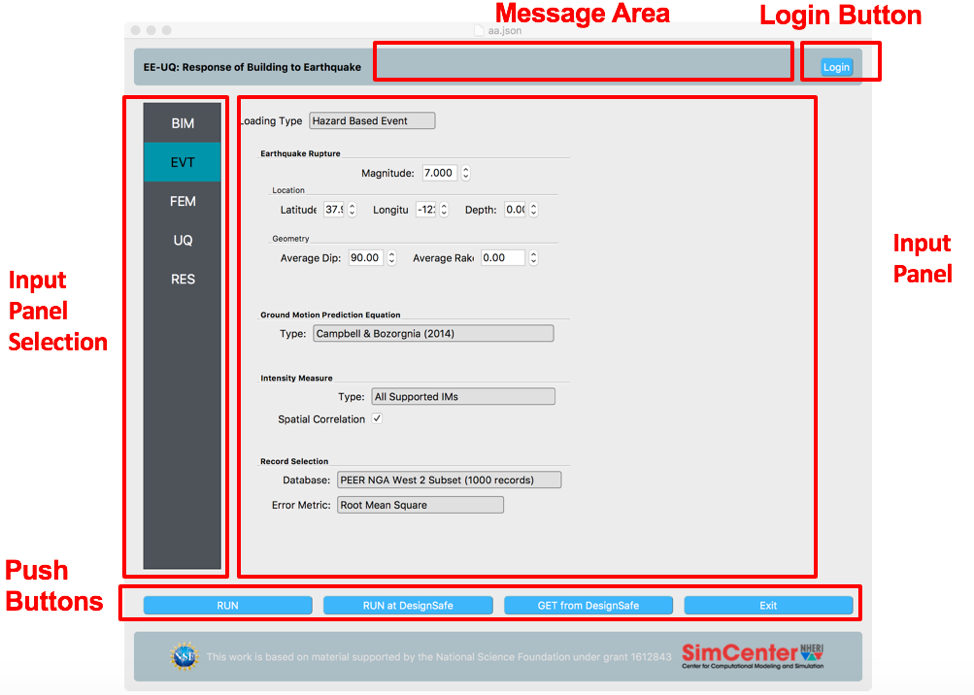
\includegraphics[width=0.8\textwidth]
    {figs/Figure1.png} }
  \caption{UI}
  \label{fig:figure1}
\end{figure}


\begin{enumerate}

\item Input Panel Selection: This  area on the left side provides the user with a selection of items to choose from from: 

\begin{enumerate}
  \item GI: General information, for specifiction of building description, location and units.
  \item SIM: Structure information model, for description of the building model.
  \item EVT: Event, for selecting the earthquake motions input.
  \item FEM: Finite element method, for specification of application and analysis options.
  \item UQ: Uncertainty quantification, for defining the distribution of the random
  variable paramaters and UQ method analysis options.
  \item EDP: Engineering demand parameters, for specification of output response quantities.
  \item RES: Results output.
\end{enumerate}

Selecting any of these will change the input panel presented.

\item Input Panel: This is the large central area of the UI that the user provides input
for the application chosen and views the results. For example if the user had selected UQ in the input panel selection, it is in this panel that the user would provide details on the distributions associated with each random variable or select the sampling method to use and provide the options necessary to run that method.

\item Push Buttons: This is the area near the bottom of the UI in which 4 buttons are presented to the user:

\begin{enumerate}
\item	RUN – to run the simulation of the user’s desktop machine.
\item	RUN at DesignSafe – to process the information, and send to DesignSafe where the job will be run on a supercomputer and results stored in your DesignSafe jobs folder.
\item	GET from DesignSafe – to obtain from DesignSafe your list of jobs and select from that list a job to download.
\item	Exit: to exit the application.
\end{enumerate}

The Screens presented to user when the first 3 of these buttons will be discussed in section 3.10.

\item Login Button: At the top right of the UI is the login button. Before the user can launch any jobs on DesignSafe they must first login to DesignSafe using their DesignSafe login and password. Pressing the login button will open up the login window for users to enter this information.

\item Message Area: In the top center of the application is the area of the interface that error and status messaged will be displayed while the application is running.

\end{enumerate}

\section{GI: General Information}
The user here provides information about the building and the units the user will work in. The widget itself presents 3 separate frames, as shown in \autoref{fig:figure2}, to the user:

\begin{enumerate}
\item Building Information frame in which user provide general information about the building, this include year of construction and type.
\item Properties frame in which user provides information about number of stories, width, depth, plan area and height of the building.
\item Location frame in which user provides location of the building. This information is used in some of event widgets to obtain events specific to the building.
\item Units frame  in which user specifies what the units will be for the inputs and outputs. Some widgets will require inputs in different units. These entries will contain units beside the specific entry to mark this.
\end{enumerate}


\begin{figure}[!htbp]
  \centering {
    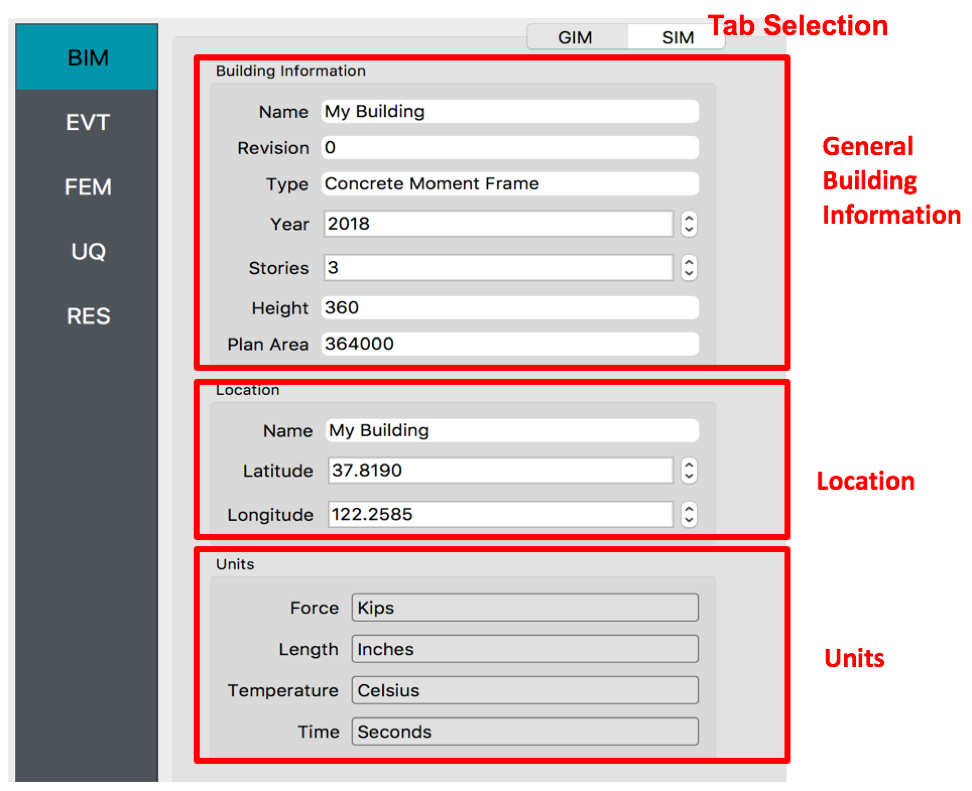
\includegraphics[width=0.8\textwidth]
    {figs/Figure2.png} }
  \caption{BIM}
  \label{fig:figure2}
\end{figure}

\section{SIM: Structural Information Model}

This panel is where the user defines the structural model of the building. The structural model is that part of the building provided to resist the lateral loads. There are a number of backend applications provided for this part of the workflow, each responsible for providing the structural analysis model to the workflow. The drop-down menu at the top of this panel is where the user selects which application to use. As the user switches between applications, the entry data changes to reflect the different inputs the different applications require. At present there are two backend applications available through the drop down menu: MDOF and OpenSees.

\subsection{MDOF}

This panel is provided for users to quickly create simple shear models of a building. The panel is divided into 3 frames:
\begin{enumerate}
\item in the top left frame the user enters the number of stories. For each story the user then enter the story height, initial stifness in 1 and 2 directions, yield strength in 1 and 2 directions, and hardeing ratio again in 1 and 2 directions. In addition user enters the floor weights and damping ratios for each of the modes.
\item In the lower left frame the user has the option of overriding an an individual floor or story basis, any of the properties set in the upper frame.
\item on the right side of the frame is a graphical widget showing the current building. When entering data into the lower left frame, those floors and stories corresponding to data being modified is highlighted in red.
\end{enumerate} 

Random Variables: Random Variables can be created by the user entering a valid string instead of a number in the entry fields for all entries except the number of floors. The variable name entered will appear as a Random Variable in the UQ panel and it is there that the user must enter the distribution for the Random Variable.


\subsection{OpenSees}
The panel is for users who have existing OpenSees model of a building that performs a gravity analysis and now wish to subject that building model to one of the EVENT options provided. The panel that presents is as shown in \autoref{fig:figure3}. The user has 3 fields that he needs to fill out:
\begin{enumerate} 
\item The user specifies the main script that contains the building model. This script should build a model and perform any gravity analysis of the building that is required before the event is applied.
\item A llist of nodes that define a column line of interest for which the responses will be determined. The column nodes should be in order from ground floor through to roof. The EDP options use this information to determine nodes at which displacement, acceleration and story drifts are calculated. 
\item An entry for the dimension of the model, i.e. 1D, 2D or 3D. This information is used to apply ground motions.
\end{enumerate}

\begin{figure}[!htbp]
  \centering {
    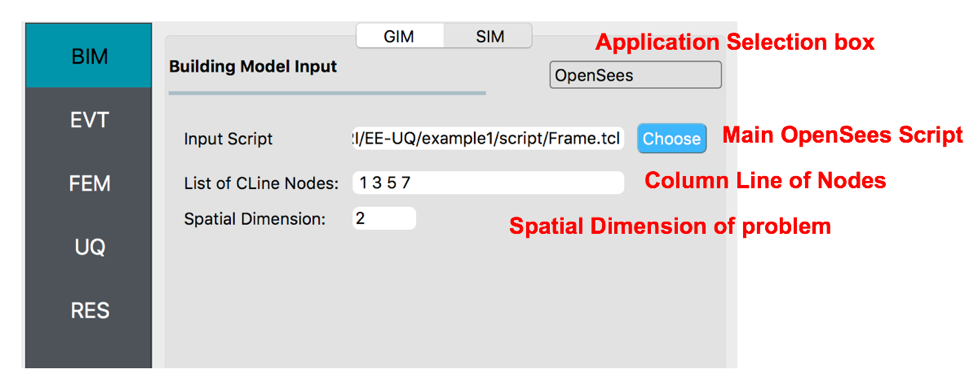
\includegraphics[width=0.8\textwidth]
    {figs/Figure3.png} }
  \caption{OpenSees Input Model}
  \label{fig:figure3}
\end{figure}

Random Variables: In OpenSees there is an option to set variables to have certain values using the pset command, e.g pset a 5.0 will set the variable a to have a value 5 in an OpenSees script. In EE-UQ any variable found in the main script to be set using the pset command will be assumed to be a Random Variable. As such, when a new main script is loaded all variables set with pset will appear as Random Variables in the UQ panel.


\section{EVT: Event}
The event panel presents the user with a drop-down menu with a list of available event applications. Event applications are applications that, given the building and user supplied data to the specific
applications input panel, will generate a list of events for the building. There are a number of options available in the pull-down menu.

\subsection{Multiple Existing}

This is provided for the user to specify multiple existing SimCenter
Event files.  If more than one event is specified it is done to provide
the UQ engine with a discrete set of events to choose from.  It is not
done with the intention of specifying that one event follows another.
The panel presented initially to the user is as shown
in \autoref{fig:figure4}.

\begin{figure}[!htbp]
  \centering {
    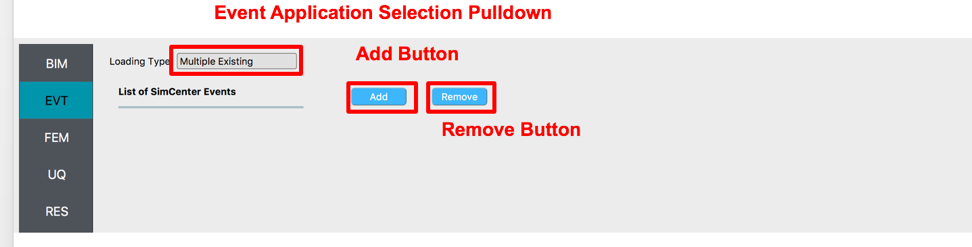
\includegraphics[width=0.8\textwidth]
    {figs/Figure4.png} }
  \caption{EVT}
  \label{fig:figure4}
\end{figure}

To add a new event, the user presses the Add button.  This adds an event to the panel.  Pressing the button multiple times will keep adding events to the panel.  \autoref{fig:figure5} shows the state after the button has been pressed twice, and data entered for the ElCentro and Rinaldi Events.

\begin{figure}[!htbp]
  \centering {
    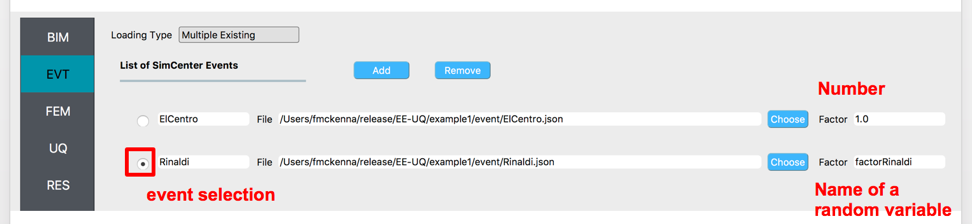
\includegraphics[width=0.8\textwidth]
    {figs/Figure5.png} }
  \caption{Adding new event}
  \label{fig:figure5}
\end{figure}


The user can enter the full path manually to the file or use the choose button,  which brings up your typical file search screen.  By default, a scaling factor of 1.0 is assigned to the event. 
The user can change this to another real value (AT PRESENT DO NOT USE INTEGER) or the user 
has the option of defining this to be a random variable by entering a name as shown for the second event. 

Note that this variable name must not start with a number, or contain any spaces or special characters, i.e. no -, +,..

The Remove button is pressed to remove events. To remove an event the user must first select
which events they wish to remove, done by clicking in the small circle at the start of the event. Once the events to remove  have been selected, the user removes all these selected evens by pressing the remove button.

If the user has multiple events to load, all the event files may first be placed by the user into a seperate folder. If the user presses the  Load Directory, the user will be able to choose a directory and the application will load all the event file (any file with a .json suffix) into the widget by choosing the directory. Initially each event will be given a load factor of 1.0.  Should the user include in that directory a file named Records.txt the application will open that file and load the events and assigned load factors from that file. Each line in Recors.txt is considered ro represent a record, and contains 2 comma seperated values: the first value being the event file and the second value the event factor. An example Records.txt is as shown below:

\begin{verbatim}
ElCentro.json,1.5
Rinaldi.json,2.0
\end{verbatim}

Random Variables: The user can, as mentioned, enter a string in the factor field to specify that the factor is to be considered a random variable. Subsequently in the UQ panel the user must provide information on the random variables distribution. Also, if multiple events are specified, the event itself will be treated as a random variable, with each event being part of the discrete set of possible events.

\subsection{Multiple PEER Event}
This is provided for the user to specify multiple existing PEER 
(\href{http://peer.berkeley.edu}{http://peer.berkeley.edu}) ground motion files. 
For PEER events the user is required to specify the individual components for the EVENTS. 
The Add/Remove buttons at the top are to create and remove an event, as per 2.2.1. 
For the PEER events the user specifies components acting in the individual degree-of-freedom directions. 
The + and – add and remove components with the remove removing all components selected. 
Each component in a PEER event can have their own scale factor, again a number or a random variable.

\begin{figure}[!htbp]
  \centering {
    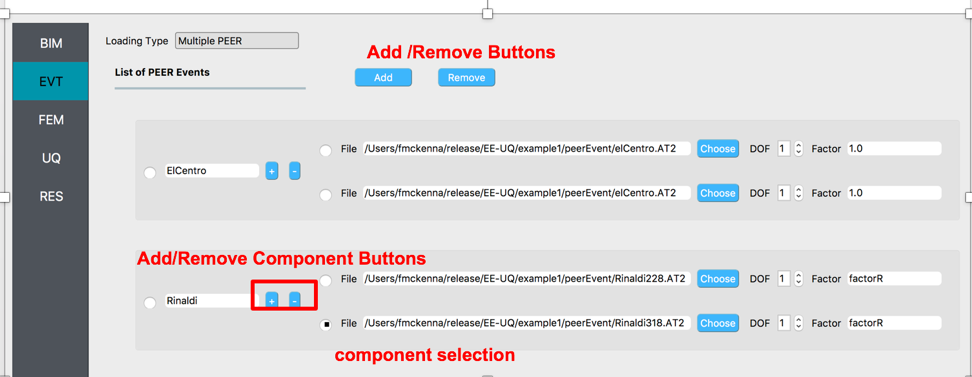
\includegraphics[width=0.8\textwidth]
    {figs/Figure6.png} }
  \caption{PEER event}
  \label{fig:figure6}
\end{figure}

If the user has multiple events to load the user can again place att the PEER .AT2 files into a separate folder and select the Load Directory option. This will allow the user to select a directory. Once selected all .AT2 files in that directory will be loaded into the application. Similar to loading multiple SimCenter events, should the user provide a file Records.txt in that directory, the application will load all files in the list and set the appropriate load factor. An example Results.txt file for multiple Peer events is as shown below:

\begin{verbatim}
elCentro.AT2,1.5
Rinaldi228.AT2,2.0
Rinaldi318.AT2,2.0
\end{verbatim}

Random Variables: The user can, as mentioned, enter a string in the factor field to specify that the factor is to be considered a random variable. Subsequently in the UQ panel the user must provide information on the random variables distribution. Also, if multiple events are specified, the event itself will be treated as a random variable, with each event being part of the discrete set of possible events.

\subsection{Hazard Based Event}
The panel for this event application is as shown
in \autoref{fig:figure7}.  This application implements a
scenario-based (deterministic) seismic event.  In this panel the user
specifies an earthquake rupture (location, geometry and magnitude), a
ground motion prediction equation, a record selection database and the
intensity measure used for record selection.  In the backend, this
application relies on three other applications to perform seismic
hazard analysis, intensity measures simulation (to create a simulated
target spectrum), and ground motion record selection/scaling.  Users
interested in learning about those applications are referred to the
documentation of the
(\href{https://github.com/NHERI-SimCenter/GroundMotionUtilities/blob/master/Readme.md}{SimCenter
ground motion utilities}).
\begin{figure}[!htbp]
  \centering {
    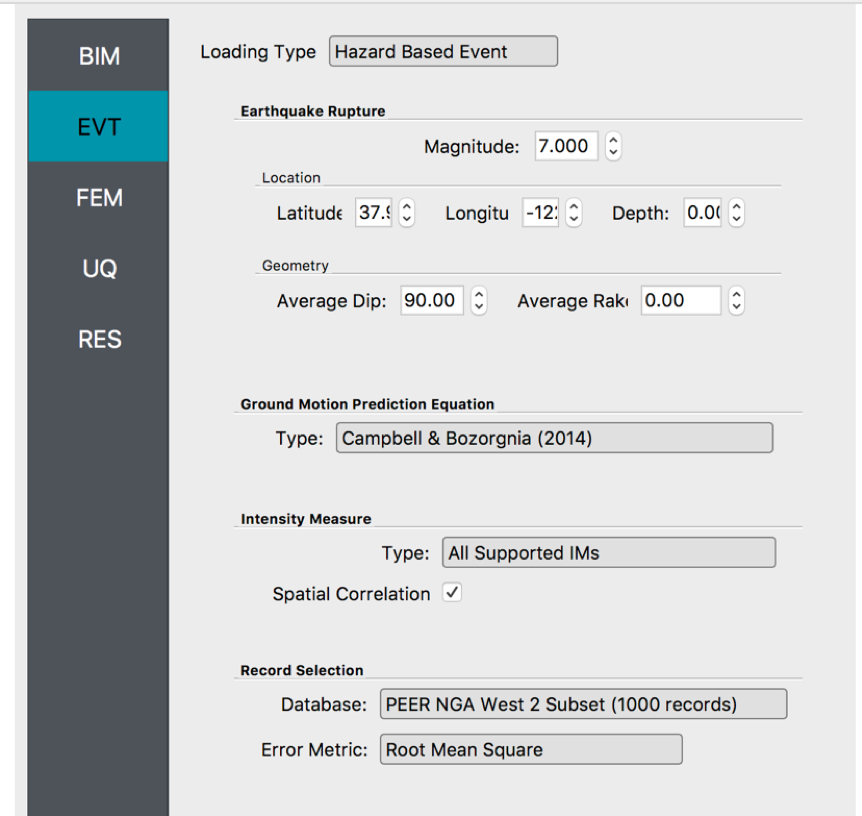
\includegraphics[width=0.8\textwidth]
    {figs/Figure7.png} }
  \caption{Hazard based event}
  \label{fig:figure7}
\end{figure}

\subsection{Stochastic Ground Motion Model}
This option allows users to generate synthetic ground motions for a
target seismic event. In order to do so, the stochastic ground motion
model is selected from the drop-down menu, as shown
in \Cref{fig:stochastic_loading}. Depending on the model selected, the
user will be asked to enter values for a number of parameters that are
used to generate a seismic event. In the current release, users can
select between the model derived by Vlachos et
al. (2018) \cite{vlachos2018predictive} and the model developed by
Dabaghi \& Der Kiureghian (2014, 2017, 2018)
[\cite{dabaghi2014stochastic}, \cite{dabaghi2017stochastic}, \cite{dabaghi2018simulation}]. Additionally,
users can provide a seed for the stochastic motion generation if they
desire the same suite of synthetic motions to be generated on multiple
occasions.  If the seed is not specified, a different realization of
the time history will be generated for each run. The backend
application that generates the stochastic ground motions relies
on \texttt{smelt}, a modular and extensible C++ library for generating
stochastic time histories. Users interested in learning more about the
implementation and design of
\texttt{smelt} are referred to its
\href{https://github.com/NHERI-SimCenter/smelt}{GitHub repository}.

All input parameters can be specified as random variables by entering
a string in the parameter field. Please note that information for the
inputs that are identified as random variables needs to be provided in
the \texttt{UQ} tab.

\begin{figure}[!htbp]
  \centering {
    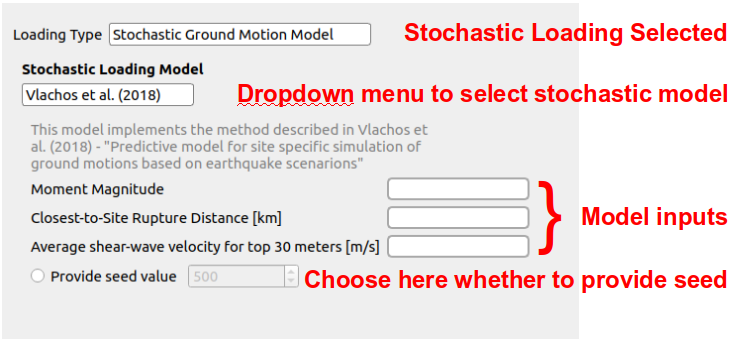
\includegraphics[width=0.8\textwidth]
    {usage/figures/stochastic_loading.png} }
  \caption{Stochastic Ground Motion Event}
  \label{fig:stochastic_loading}
\end{figure}




\subsubsection{s$^3$hark}
The panel for this event application is as shown in \autoref{fig:s3hark0}. 
This application does effective free-field site response analysis of a soil column.
In this panel the user specifies a ground motion at the bottom of the column. 
With soil layer properly defined, the motion at the ground surface will be given at the end of the analysis.
\begin{figure}[!htbp]
  \centering {
    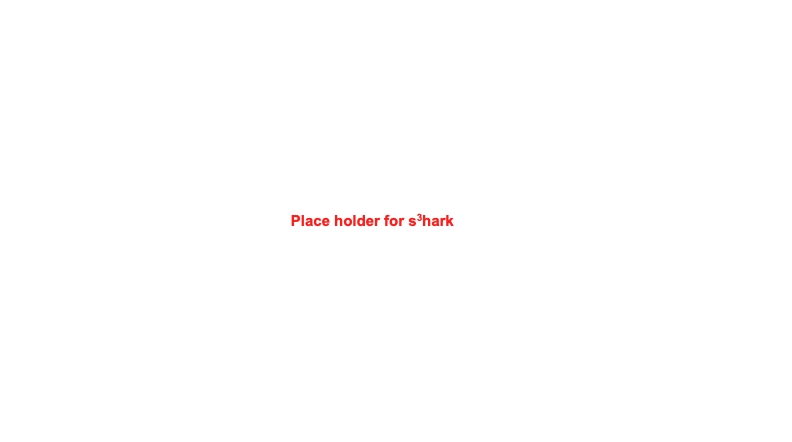
\includegraphics[width=0.8\textwidth]
    {figs/s3hark0.png} }
  \caption{s$^3$hark}
  \label{fig:s3hark0}
\end{figure}

The UI of s$^3$hark is shown in \autoref{fig:s3hark1}.
There are two graphics shown in the left of the panel. The first one is the soil column graphic, 
which shows a visualization of the soil column.
The second one is the mesh and profile graphic, 
which shows the finite element mesh and profile plots.
On the right of the panel are operation area, soil design table, configure tab, layer property tab and response tab. 


\begin{figure}[!htbp]
  \centering {
    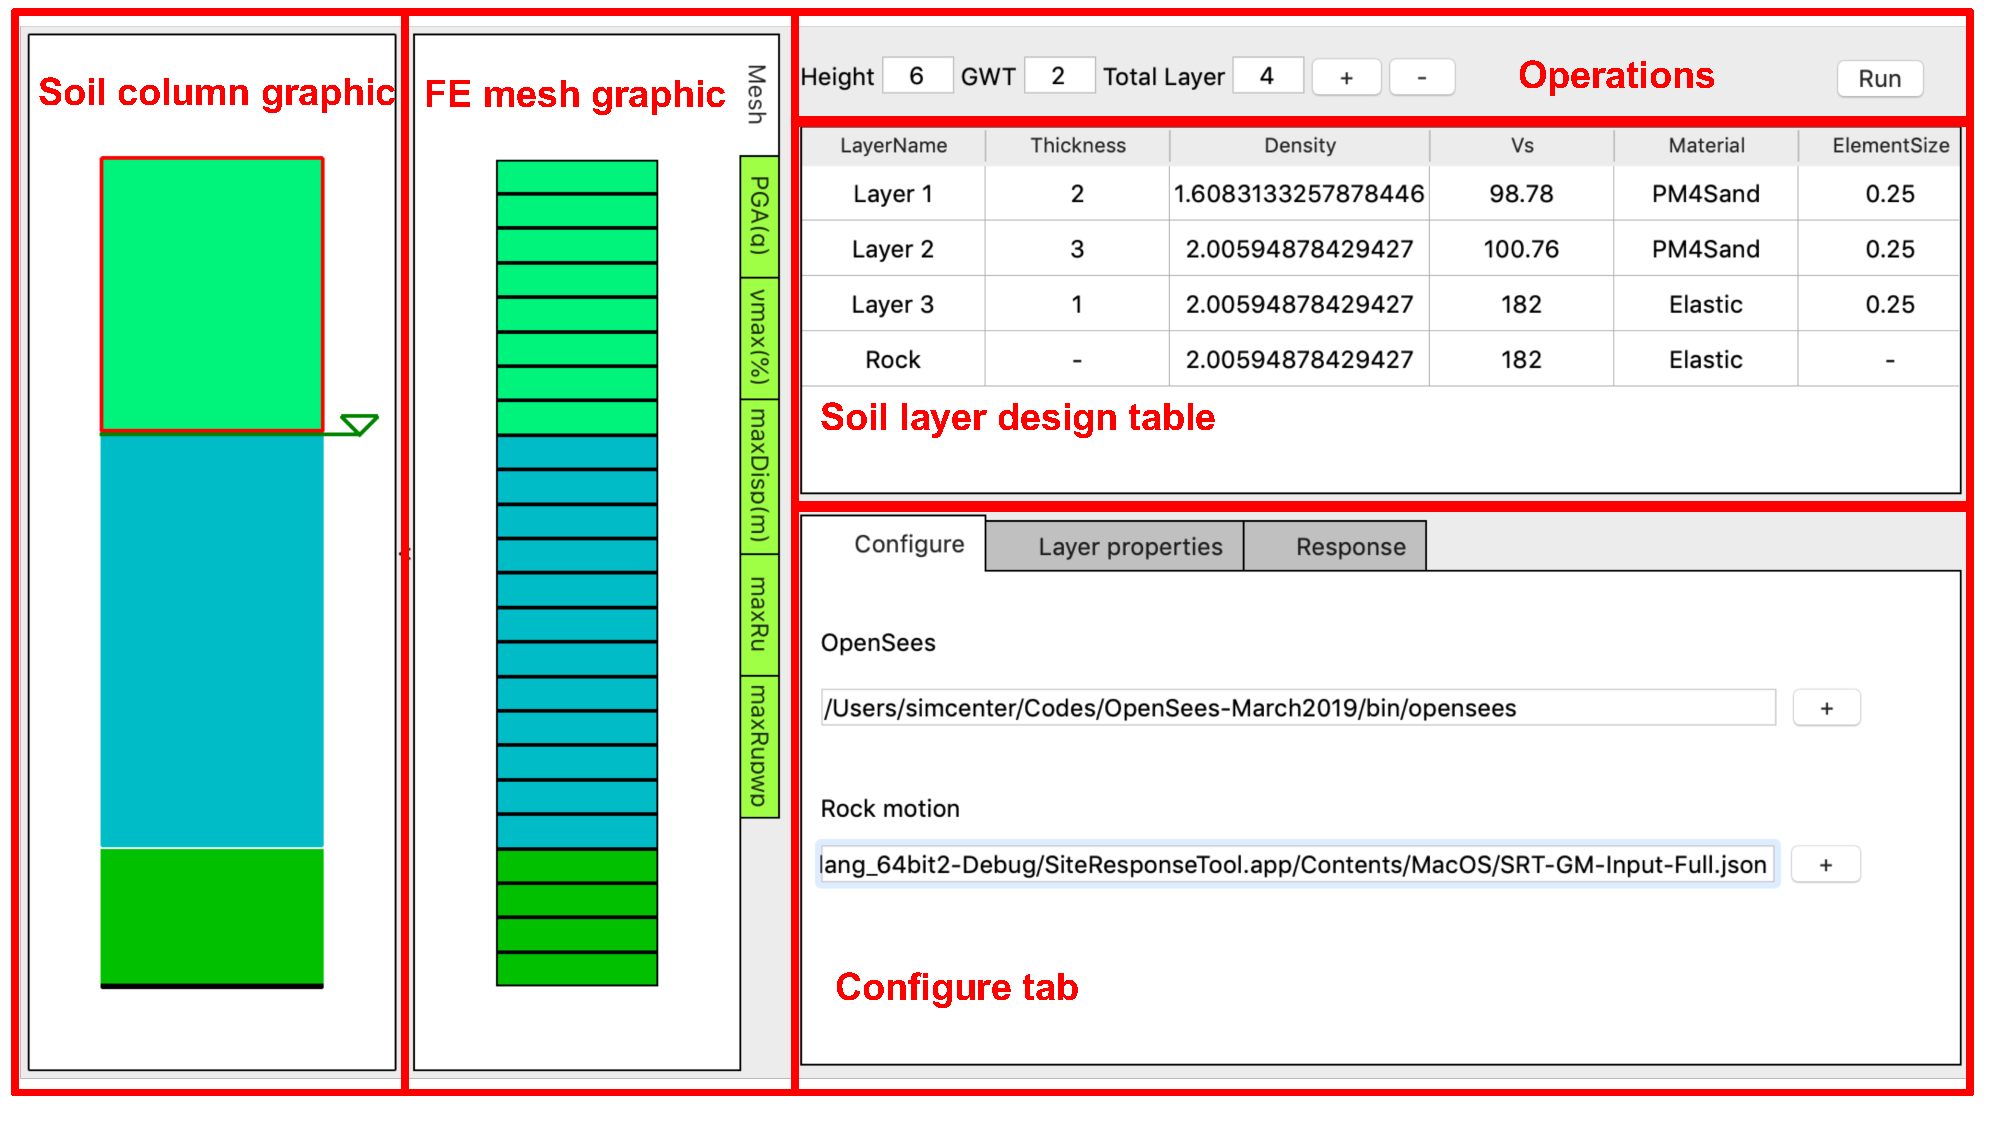
\includegraphics[width=0.8\textwidth]
    {figs/s3hark1.pdf} }
  \caption{s$^3$hark - Panels}
  \label{fig:s3hark1}
\end{figure}

In the operation area as shown in \autoref{fig:s3hark2}, click the plus button to add a layer and the minors button to delete a selected layer. 
Change the ground water table in the GWT input field. 
In the configure tab, path of OpenSees executable and rock motion file need to be specified.
A click on the run button will start the finite element analysis.


\begin{figure}[!htbp]
  \centering {
    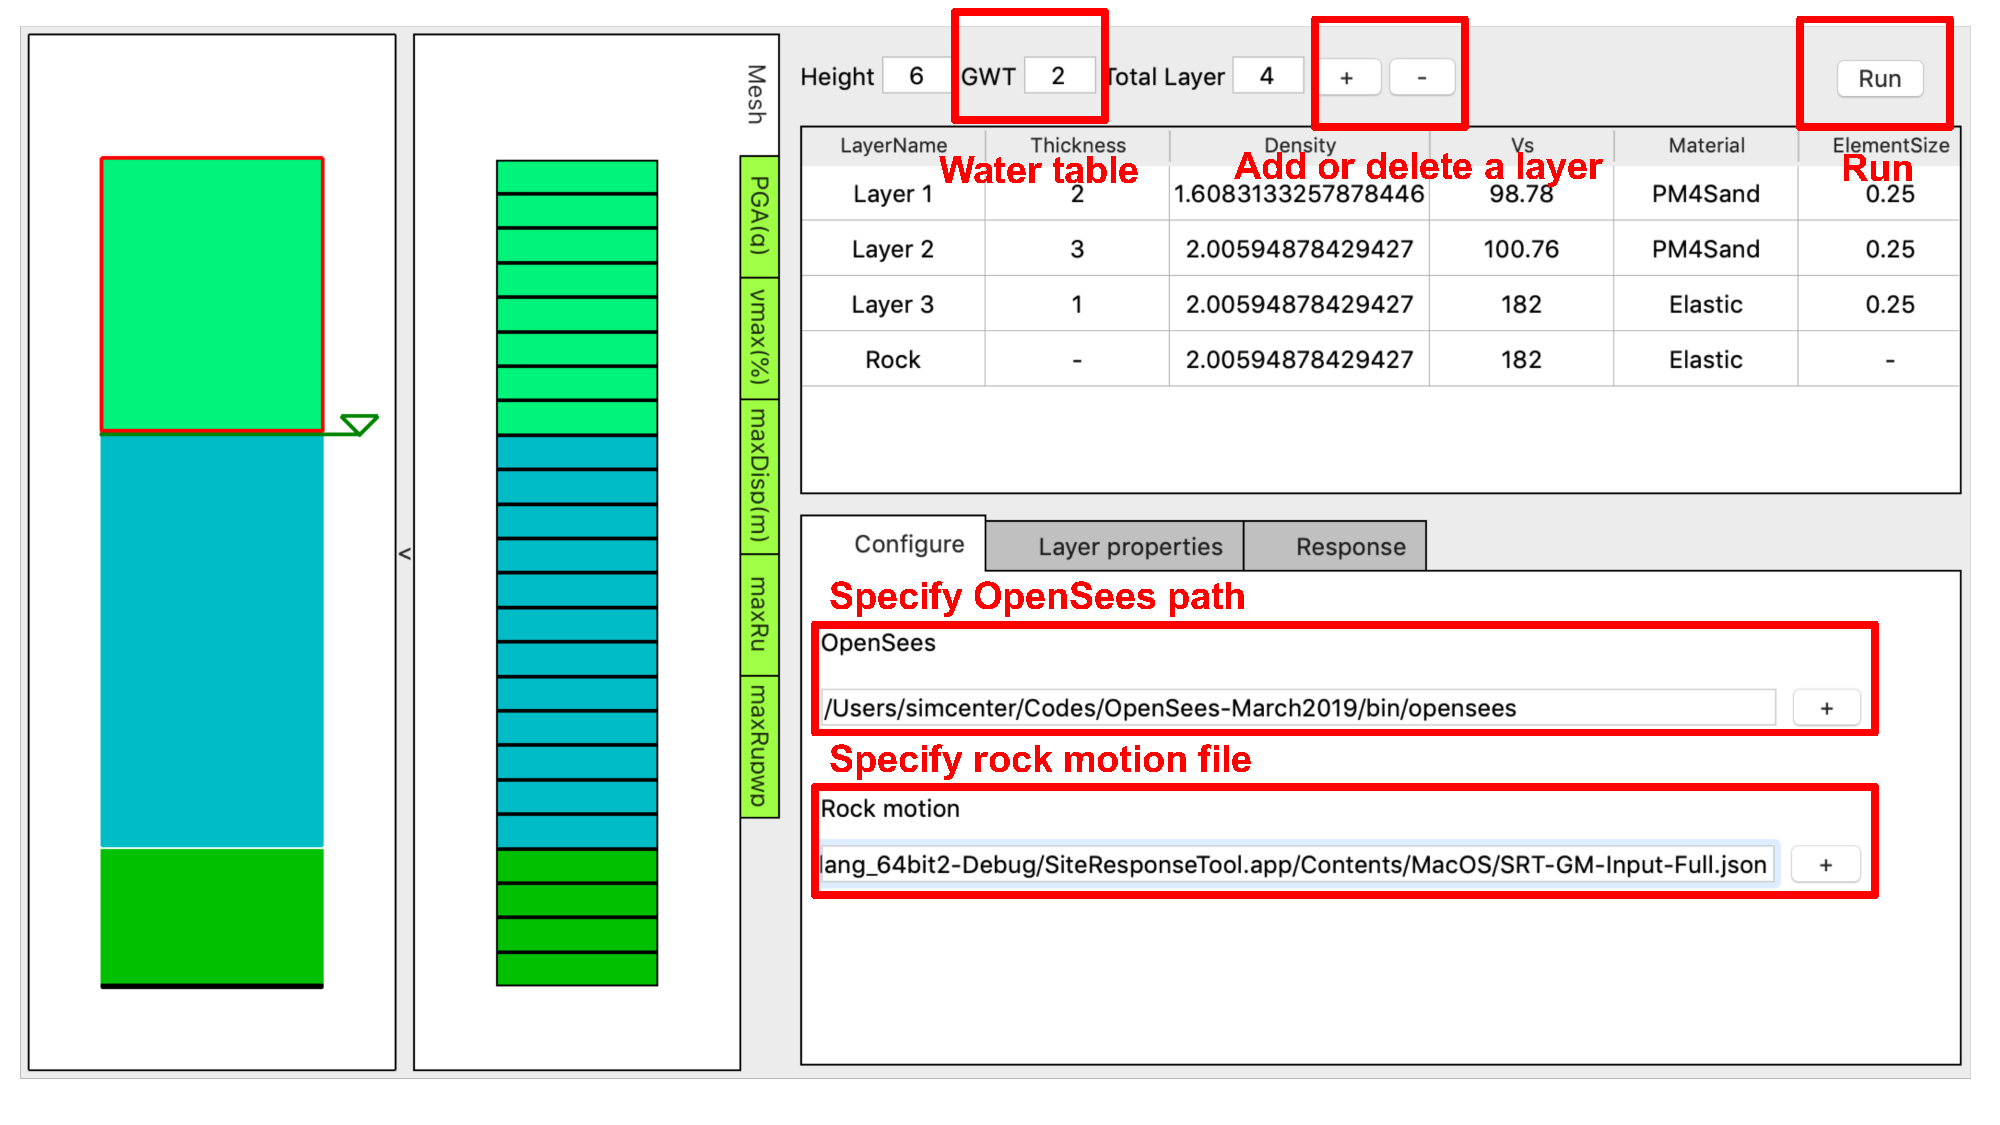
\includegraphics[width=0.8\textwidth]
    {figs/s3hark2.pdf} }
  \caption{s$^3$hark - Configurations and Operations }
  \label{fig:s3hark2}
\end{figure}

Either click on the soil column or the table to select a layer \autoref{fig:s3hark3}. 
When a layer is selected, it will be highlighted in both the soil column graphic and the table. 
Selection of a soil layer will invoke the Layer properties tab, where the user can specify the material properties of this layer.
Double click on a cell of the table will allow the user to change the corresponding value.

\begin{figure}[!htbp]
  \centering {
    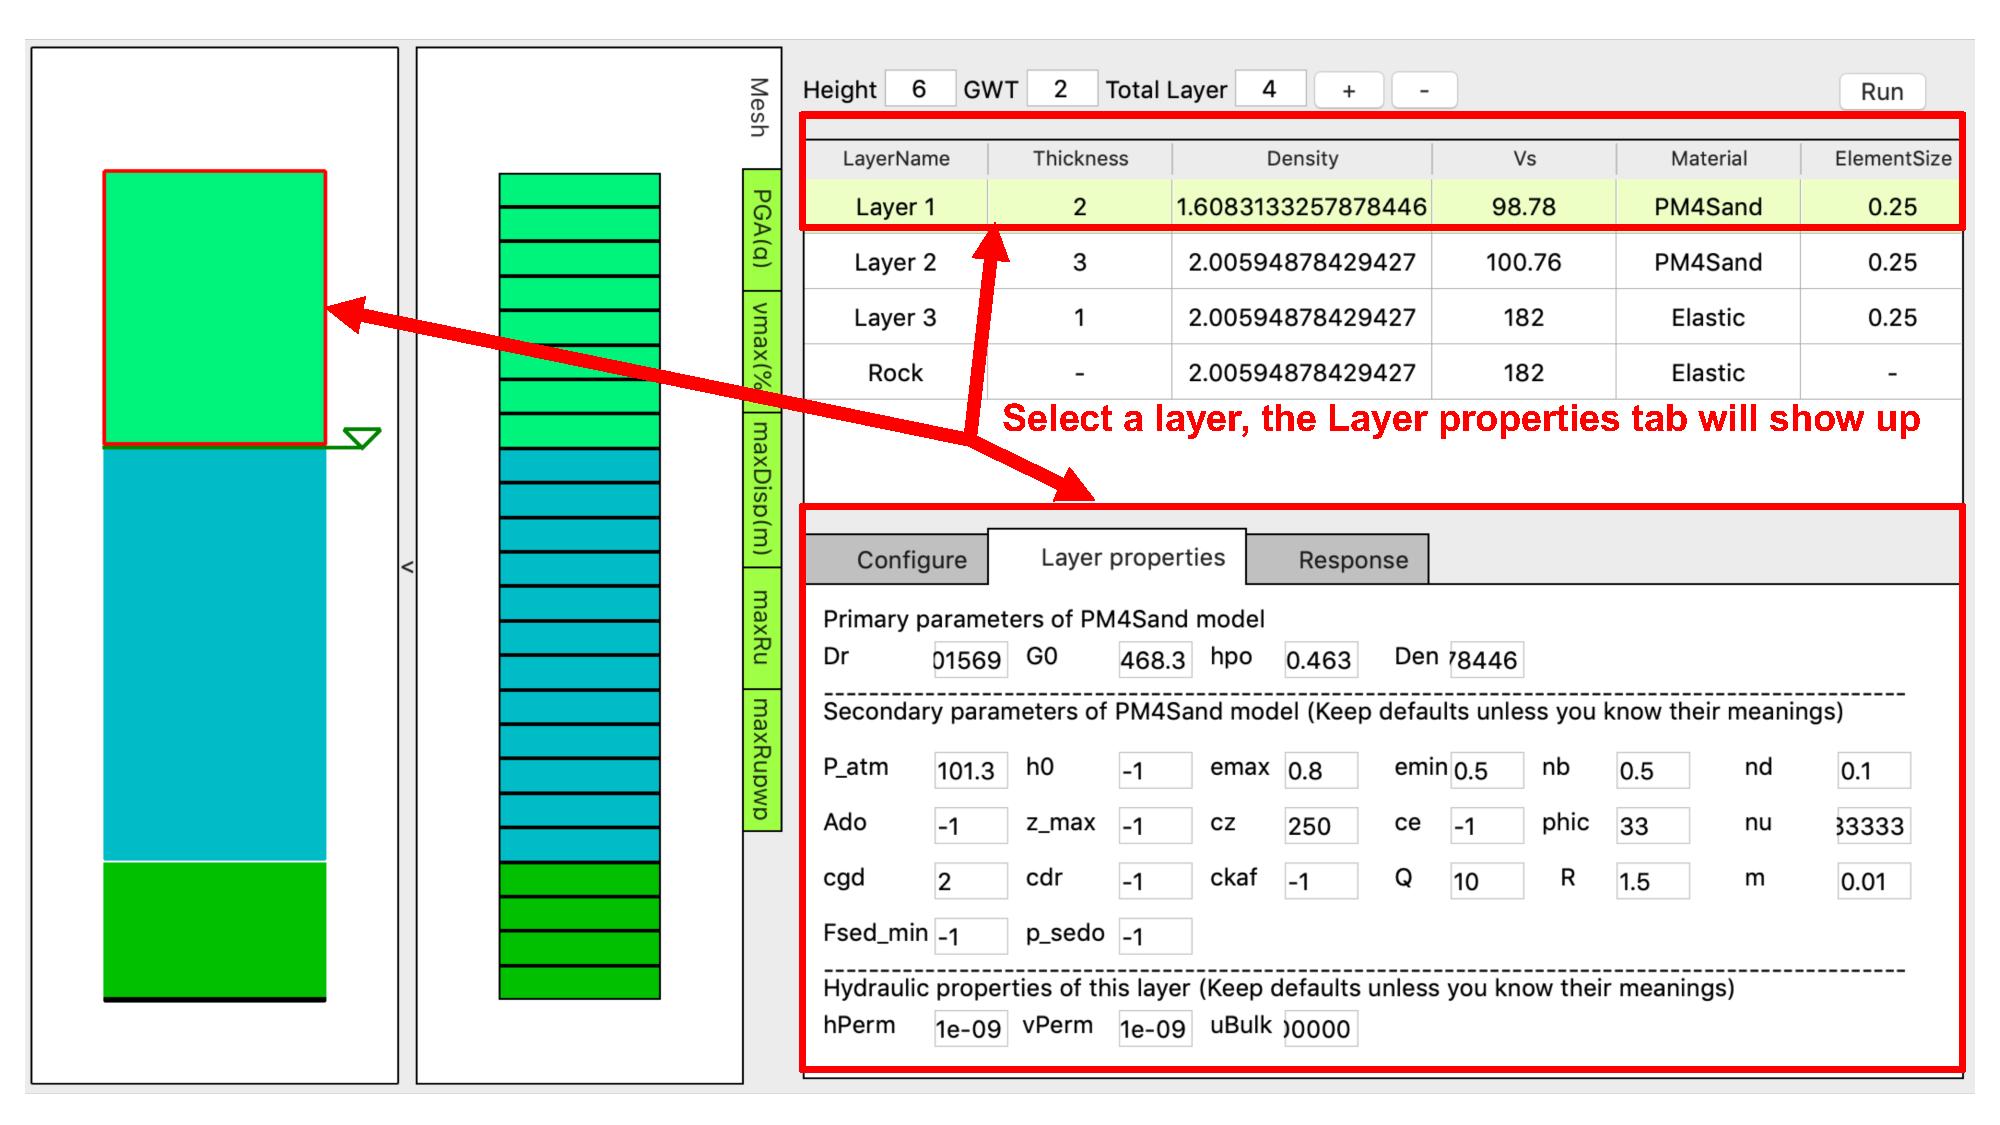
\includegraphics[width=0.8\textwidth]
    {figs/s3hark3.pdf} }
  \caption{s$^3$hark - Layer modification }
  \label{fig:s3hark3}
\end{figure}


Upon the finish of the finite element analysis, the ground motion at the soil surface (\autoref{fig:s3hark4}) will be stored in EE-UQ's input file.
This computed motion will be later applied to the bottom of the building.

\begin{figure}[!htbp]
  \centering {
    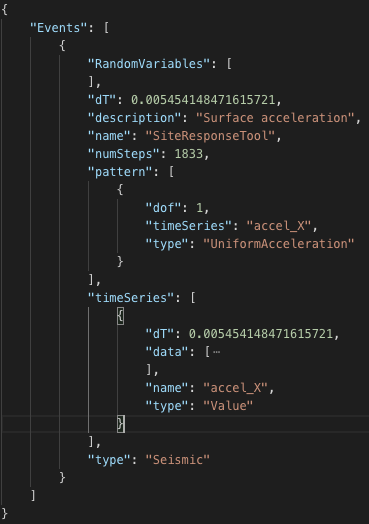
\includegraphics[width=0.4\textwidth]
    {figs/s3hark4.png} }
  \caption{s$^3$hark - Surface motion }
  \label{fig:s3hark4}
\end{figure}












\subsection{User Application}
The final selection option is a user specific application. 
The user specifies the application name and the input file containing the specific input information 
needed by the application when it is running in the backend. 
As will be discussed, the user is also required when they use an additional application not provided, 
to edit the tools registry file. Here they must include a new event application with this same name 
and the location where that application can be found relative to the tools application directory. 
If running on DesignSafe, that application must of course be built and available on the Stampeded2 supercomputer. 
NOTE that given how DesignSafe runs the applications through Agave, this applications file permissions must be 
world readable and executable (as when user running their application through DesignSafe and Agave, they are not running as themselves!)

\begin{figure}[!htbp]
  \centering {
    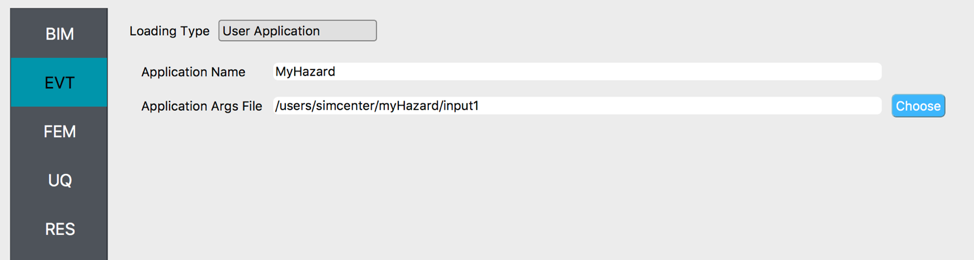
\includegraphics[width=0.8\textwidth]
    {figs/Figure8.png} }
  \caption{User defined event}
  \label{fig:figure8}
\end{figure}


\section{FEM: Finite Element Method}
The FEM panel is intended to present users with a selection of FEM applications that will take a building model generated by the BIM application and the EVENT from the event application and perform a deterministic simulation. 
At present there is only one application available, OpenSees and there is no application selection box.  That will be modified in future versionsto allow user to provide their own simulation application.  This is not the standard OpenSees executable, but consists of a pre- and post-processor to take the  BIM and EVENT file and use OpenSees to determine the response, returning these responses in an EDP. 

For the OpenSees application the user is required to specify the options to be used in the transient analysis. As shown in the figure this includes the choice of 
\begin{enumerate}
\item Solution algorithm, the default is Newton Raphson.
\item Integration Scheme, the default is Newmarks linear acceleration method.
\item Convergence Test, the default is a norm on the unbalance force.
\item Convergence tolerance
\item Damping Ratio.
\end{enumerate}

All the options available can be found in the OpenSees online user manual.\\

A default transient analysis script is run with these inputs. It is built for Version 3.0.0+ of OpenSees and uses a divide and conquer  algorithm in event of a convergence failure issue. This new algorithm does not always work. \\

The user is also able to specify their 
own analysis script to run instead of the default. When chosen the variables numStep and dt that are obtained from the EVENT are set by the program. These variables can be used by the user when providing their own analysis script.

\section{UQ}
Throughout the input specification the user is defining variables. As described in the above sections many of these variables can be specified by the user to be random variables with a distribution on their values. It is in the UQ panel that the user specifies what these distributions are. 
It is also here that the user specifies the UQ method and the input values are for these UQ methods. 
The panel is split,  as shown in \autoref{fig:figure10}, into 2 frames:
 \begin{enumerate}
\item Sampling Methods 
\item Random Variables
\end{enumerate}

\begin{figure}[!htbp]
  \centering {
    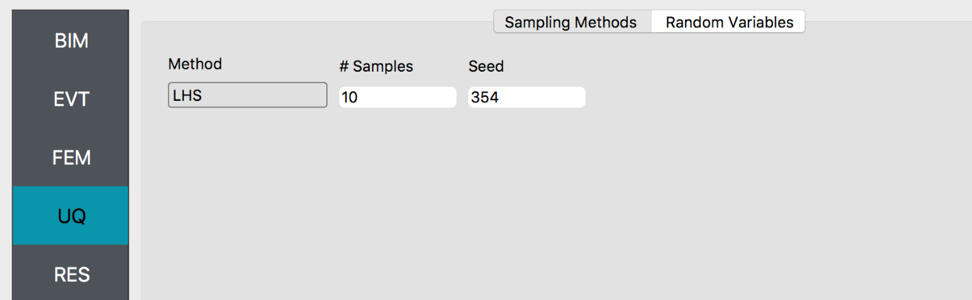
\includegraphics[width=0.8\textwidth]
    {figs/Figure10.png} }
  \caption{UQ}
  \label{fig:figure10}
\end{figure}


\subsection{Sampling Methods}
In the sampling methods the user selects the sampling method to use from the method dropdown. Currently this is limited to two options: 
Monte Carlo and Latin Hypercube Sampling (LHS). For the one selected, the user specifies the number of simulations to be perform and the seed.

\subsection{Random Variables}
The Random Variable panel is where the user enters the random variables. Each random variable has a name and a distribution. The distribution is selected frm the drop-down menu. By changing the distribution type, the inputs required to define the distribution change. The following are the list of distributions available:
\begin{enumerate}
\item Normal
\item Lognormal
\item Beta
\item Uniform
\item Weibull
|item Gumbell
\item UserDef
\end{enumerate} 

As with other panels, the random variables can be added or removed. Care must be taken by the user in ensuring that if the user removes random variables from this panel that they also remove them from the other input widgets. Failing to do so may result in the program faling to complete.


\begin{figure}[!htbp]
  \centering {
    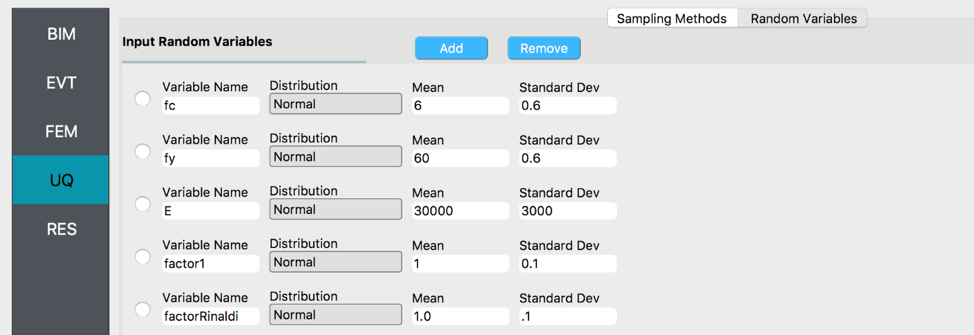
\includegraphics[width=0.8\textwidth]
    {figs/Figure11.png} }
  \caption{Random variables}
  \label{fig:figure11}
\end{figure}

\section{EDP: Engineering Demand Parameters}
This panel is where the user selects the outputs to be displayed when the simulation runs. There are two options available in the pull-down menu:
\begin{enumerate}
\item Standard Earthquake
\item USer Defined
\end{enumerate}

\subsection{Standard Earthquake}
When the user selects standard Earthquake there are no additional inputs required. The standard earthquake EDP generator will ensure the the max absolute value of the following are obtained: \begin{enumerate}
\item Relative Floor displacements:
\item Absolute Floor Accelerations
\item Interstory Drifts
\end{enumerate}

The  results will contain results for these in abbreviated form:
\begin{itemize}
\item PFD peak relative floor displacement $1-PFD-FLOOR_CLINE$
\item PFA peak floor acceleration (relative + ground motion): $1-PFA-FLOOR-CLINE$
\item PID peak inter-story drift: $1-PID-STORY-CLINE$
\end{itemize}

\subsection{User Defined}
This panel allows the user to provde to determine their own output and process it. When using this option the user provides additional data:
\begin{enumerate}
\item Additional Input: These are additional commands that are invoked by the analysis application before the transient analysis is performed. For example, foe OpenSees this would be a script containing a series of recorder commands.
\item Postprocess Script: This is a python script that will be invoked after the finite element application has run. It must be provided by the user. It's purpose is to process the output files and create a single file, results.out. This file must contain a single line with as many entries as EDP's specified.

\item Response Parameters. This is an area in which the user associates a variable name with the column of the results output file. If the process script has an array of strings named named EDP's the script, the Response Parameters will be initially set with these values from the script.
\end{enumerate}


\section{RES}

When the user hits the Run button, and assuming the results are successful. The results are presented here.  A successful run or download of a job that ran successfully will result in 3 tabbed widgets being displayed in this panel.  The first panel shows summary statistics: mean and stdDev values or min-max values if discrete set, i.e. multiple events for each of the EDP's specified in the EDP panel.

\begin{figure}[!htbp]
  \centering {
    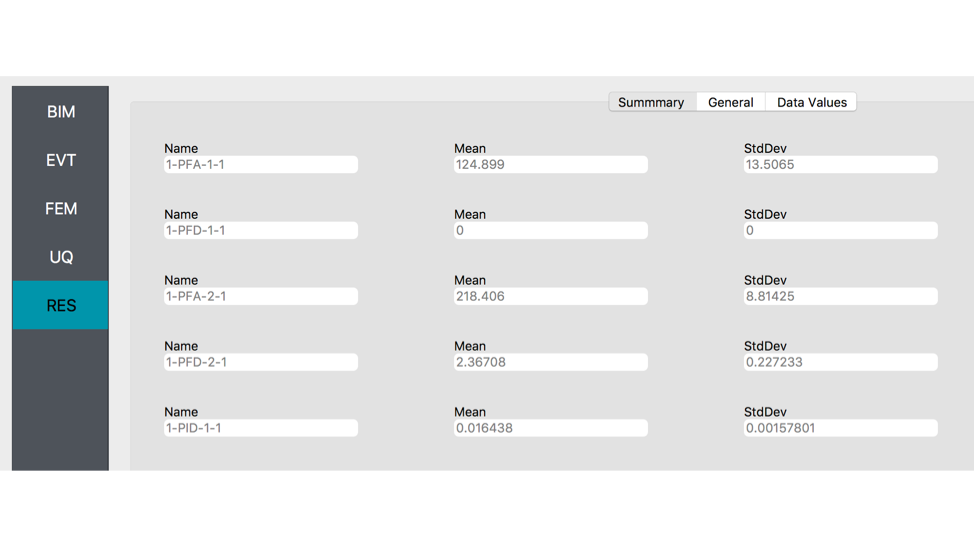
\includegraphics[width=0.8\textwidth]
    {figs/Figure12.png} }
  \caption{RES}
  \label{fig:figure12}
\end{figure}

The second panel shows the summary information.

\begin{figure}[!htbp]
  \centering {
    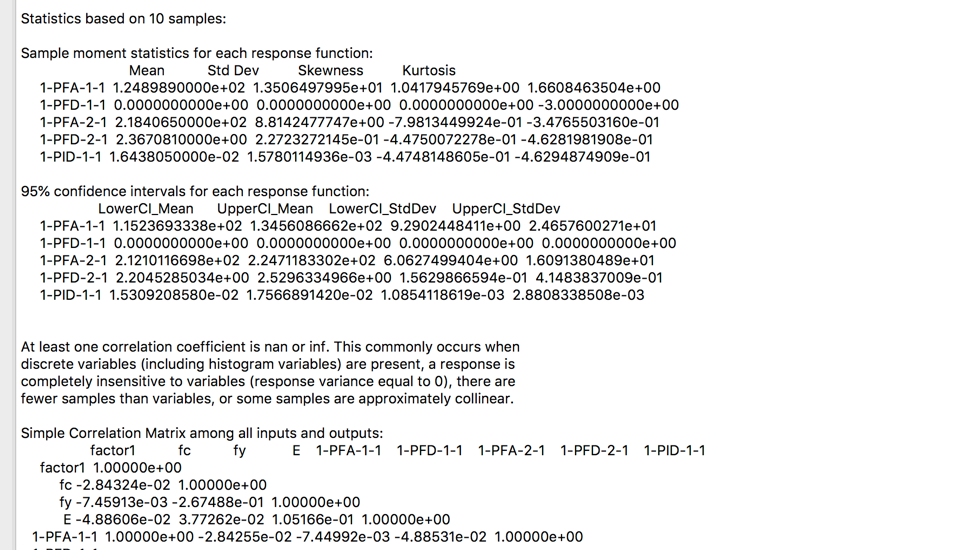
\includegraphics[width=0.8\textwidth]
    {figs/Figure13.png} }
  \caption{RES General tab}
  \label{fig:figure13}
\end{figure}

The third panel presents graphically and in tabular form the results. By selecting different columns with left and right mouse buttons in the table below the graphic, 
the information in the graph is changed. Selecting the left mouse button changes the Y axis, the right mouse changes the X axis. If the same column is selected 
using both left and right keys, the CDF and PDF is displayed. If last mouse press was with the left button, the PDF and if right the CDF.

As for the columns. You will see a column for each random variable the workflow came across. There may be more than you specified if the applications want the 
UQ engine to consider their own variables in the computation. The outputs at present are limited to:



\begin{figure}[!htbp]
  \centering {
    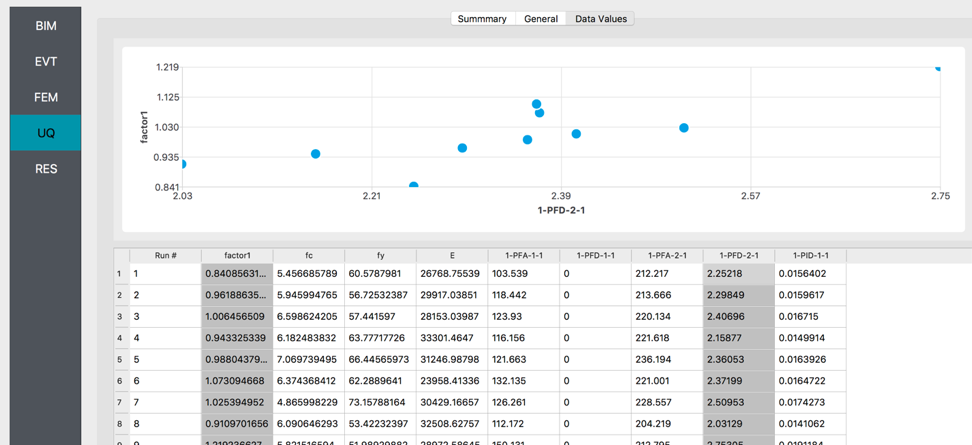
\includegraphics[width=0.8\textwidth]
    {figs/Figure14.png} }
  \caption{UQ Data Values}
  \label{fig:figure14}
\end{figure}



\section{Push Buttons}
There are a number of buttons in the Push Button area of \autoref{fig:figure1}:
\subsection{RUN – to run the simulation of the user’s desktop machine.}
\begin{figure}[!htbp]
  \centering {
    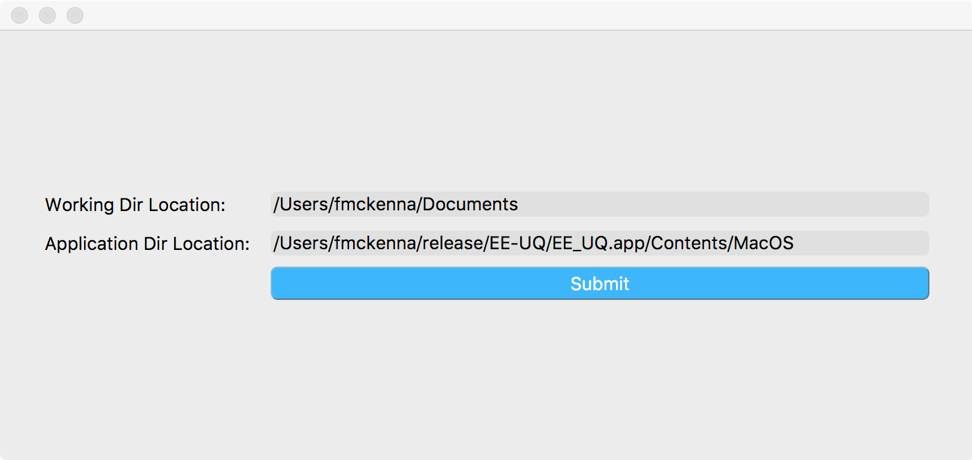
\includegraphics[width=0.8\textwidth]
    {figs/Figure15.png} }
  \caption{Run button}
  \label{fig:figure15}
\end{figure}
The window that pops up is as shown in \autoref{fig:figure15}. There are 2 entries and a push button: 

\begin{itemize}
\item Working Dir Location: specifies where the $EE_UQ$ application can create a “temporary” directory called tmp. SimCenter that the application 
creates when the submit button is pressed. The application creates this directory, copies files to it that the application needs as a result of your 
input (e.g. if you are using OpenSees input script, it will to the tmp. SimCenter directory copy that script, ALL FILES IN THAT DIRECTORY AND ALL FILES IN 
SUBDIRECTORIES OF THAT DIRECTORY GET COPIED SO DON’T PLACE THE SCRIPT IN HOME, DOWNLOADS, DOCUMENTS, ….
\item Application Dir Location: SHOULD NOT BE TOUCHED unless you are introducing your own applications or want to build and modify the 
applications provided with the tool. It is this directory the application tool looks to find the applications to run.
\end{itemize}


Finally, when inputs are finished the user hits submit button to start the backend job. If it runs the window will close and the RES 
panel will pop up on successful run. Do not press the submit button multiple times while waiting for it to close. We cannot guarantee 
what will happen and we did not disable the button in this release.

\subsection{RUN at DesignSafe}
Click this button to process the information, and send to DesignSafe where the job will be run on a supercomputer and results stored in your DesignSafe jobs folder.

\begin{figure}[!htbp]
  \centering {
    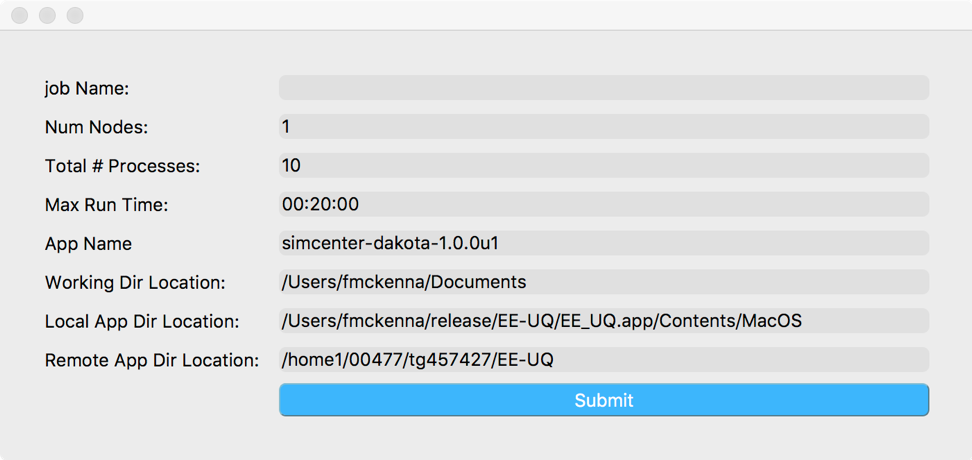
\includegraphics[width=0.8\textwidth]
    {figs/Figure16.png} }
  \caption{Remote button}
  \label{fig:figure16}
\end{figure}

A similar bit longer input panel is brought up:
\begin{itemize}
\item JobName: The name the user can use to identify the job in Get from DesignSafe.
\item NumNodes: The number of compute nodes to use on Stampede2. Using the default App Name the job will run on Stampede2’s KNL Landing (KNL) 
compute nodes. Each node has 68 cores. The actual number of cores the application will use on each of these nodes depends on the total number of 
processes specified. As per the TACC webpage, for MPI tasks it’s best not to specify more than 64-68 processes to run. Depending on the numerical 
computations and amount of memory each uses, so as to avoid page faulting, for large simulations you may wish to use more nodes and less processes.
\item Total Number of Processes: Total number of MPI parallel processes the UQ engine is going to use.
\item Max Wall Time:  HOURS:MIN:SEC be conservative. Your job is killed after the time limit. On Stampede2 you have a max wall time of 24 hours.
\item App Name:   Name of Agave app to run. DO not touch unless you know what you are doing.
\item Working Dir Location: specifies where the $EE_UQ$ application can create a “temporary” directory called tmp. SimCenter that the application 
creates when the submit button is pressed. The application creates this directory, copies files to it that the application needs as a result of your 
input (e.g. if you are using OpenSees input script, it will to the tmp. SimCenter directory copy that script, ALL FILES IN THAT DIRECTORY AND ALL FILES 
IN SUBDIRECTORIES OF THAT DIRECTORY. (SO, DON’T PLACE THE SCRIPT IN HOME, DOWNLOADS, DOCUMENTS, …). That directory is removed when jib has been successfully submitted.
\item Local App Dir Location: SHOULD NOT BE TOUCHED unless you are introducing your own applications or want to build and modify the applications 
provided with the tool. It is this directory the application tool looks to find the applications it needs.
\item Remote App Dir Location: Remote directory on Stampede2 where applications needed by workflow reside. DO not touch unless you know what you are doing.

\end{itemize}


\subsection{GET from DesignSafe}
	Click this button to obtain from DesignSafe your list of jobs and select from that list a job to update status of, download or delete.

\subsection{Exit}
Click this button to exit the application. 


\chapter{Theory and Implementation}
\label{chap:theory}
The following section describes the workings of the tool. If you intend to use the tool a lot or extend it, 
it is important that you read this section. Some Definitions before we start:
\begin{itemize}
\item Workflow: A sequence of steps involved in moving from a beginning state to an ending state.
\item Scientific Workflow Application: An application that automates a workflow process through software, with each step in the 
workflow being performed by a separate “scientific” software application.
\item Scientific Workflow System software providing an infrastructure for the set-up, scheduling, running, and monitoring of a 
user defined scientific workflow application. 
\end{itemize}

The EE-UQ application is a very limited scientific workflow system that allows users to create scientific workflow applications needed for the characterization of the response of a building subjected to earthquake ground motions. It allows the users to then create and run the workflow application using the data of the users choosing. The application itself is composed of 2 parts:

\begin{itemize}
\item	Frontend User Interface (UI): This is the application the user interacts with to create a building description, the BIM, and specify  the workflow to run, i.e. given the building, the user chooses which applications to use and what data to use for the different applications. 
The UI is what was explained in section 3. It’s purpose, as is shown in \autoref{fig:figure17}, is to create the BIM and start the workflow. 
Currently the inputs for the workflow are stored in the BIM file to reduce file overhead.
\item	Backend Application: This is the application that actually creates and runs the workflow. It consists of a script that processes the output file from the UI to determine the applications to run and their data, it invokes these applications using the outputs from one application as the input to another. The application that is run is a python script, EE-UQ.py, that can be found in the /applications/Workflow/ directory. 
The input and output from each application is in the form of JavaScript Object Notation (JSON) files. JSON is a human readable file format used  widely for passing data between your front-end browser application (Safari, Firefox, Internet Explorer) and backend servers.
\end{itemize}



\begin{figure}[!htbp]
  \centering {
    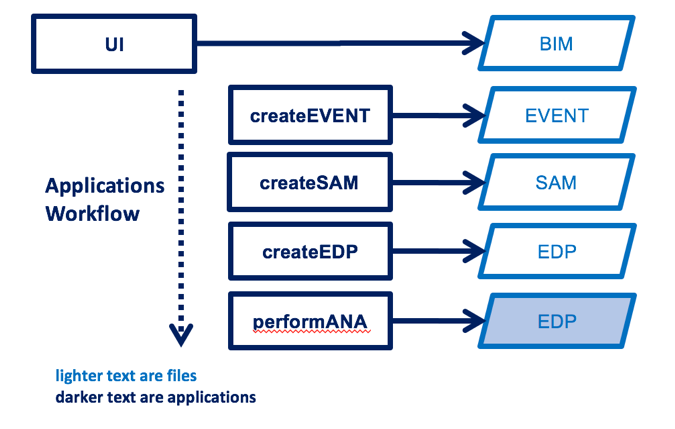
\includegraphics[width=0.8\textwidth]
    {figs/Figure17.png} }
  \caption{Workflow}
  \label{fig:figure17}
\end{figure}


In the absence of uncertainty, the applications that are invoked by this script are categorized into certain types of applications and are as shown in \autoref{fig:figure17}:
\begin{enumerate}
\item	 createEVENT: given the structure and the user input for hazard application, define the loadings for the building, i.e. the ground motions for an earthquake event. The output file is an EVENT file.
\item	 createSAM: given the building description and event, create a finite element model of the building. The output file is a SAM (Structural Analysis Model) file.
\item	 createEDP: given the building, determine what output quantities are required. The output file is the EDP (engineering Demand Parameters) file.
\item	 Currely the user has no selection over the EDP’s as the StandardEarthquakeEDP application is the built-in default application.
\item	 performANA: given the finite element model and the event, perform a finite element simulation. The responsibility of the performANA is to fill in the values in the EDP files.
\end{enumerate}


The need to characterize the uncertainties in the computed response complicates this workflow. This is because the uncertainties in the inputs, 
random variables and random field variables, may exist for each application, e.g. Young’s modulus in the building input file, magnitude of event or 
event ground motion in createEVENT, finite element material properties in createSAM, and integration scheme, damping ratio or convergence tolerance in performANA. 

\begin{figure}[!htbp]
  \centering {
    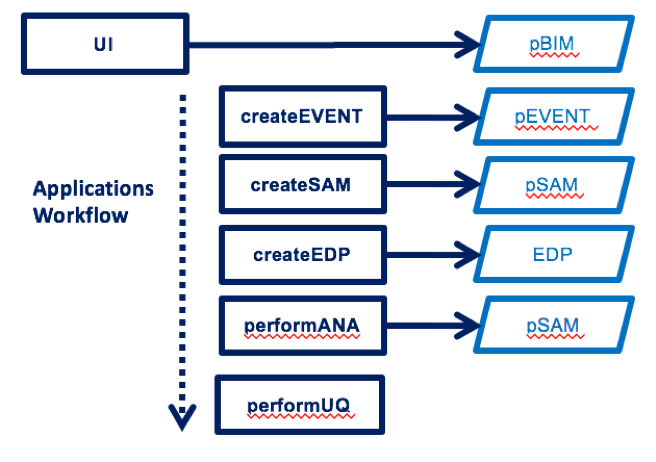
\includegraphics[width=0.8\textwidth]
    {figs/Figure18.png} }
  \caption{Workflow}
  \label{fig:figure18}
\end{figure}

As a consequence, each application is called with 2 different sets of input arguments. The first time the application is invoked with a “–getRV” 
input argument. This tells the application to return information about the random variables inside a “randomVariables” entry in the p output file 
generated by the application along with other needed data, e.g. the event type. The randomVariables is a JSON array of random variables, each with a field for a name, a type, a value, and other info that depends on the type, e.g. \\ \\


\begin{lstlisting}
{
  "randomVariables": [
        {
            "distribution": "Normal",
            "mean": 6,
            "name": "fc",
            "stdDev": 0.6,
            "value": "RV.fc",
            "variableClass": "Uncertain"
        },
        {
            "distribution": "Normal",
            "mean": 60,
            "name": "fy",
            "stdDev": 6,
            "value": "RV.fy",
            "variableClass": "Uncertain"
        },
        {
            "distribution": "Normal",
            "mean": 30000,
            "name": "E",
            "stdDev": 3000,
            "value": "RV.E",
            "variableClass": "Uncertain"
        }

}
\end{lstlisting}


It is during the running of the UQ engine that the value field in these random variables are filled in. Initially as shown, the value field contains RV.variableName. 
This is a must and what is used by the UQ engine to set the value. It is when the application is called again by the UQ engine during it’s running that the a
pplication is called without the “-getRV”. The application finds these value fields now set to numbers (or strings) in the pFiles that the application uses. \\

The performUQ application is actually a script that calls 3 applications, as shown below:
\begin{enumerate}
\item	 PreProcessUQ: will first must parse all the pFiles to build the list of all random variables.
\item	 PeformUQ: It then invokes the UQ engine, which for the number of samples specified will fill in the random variable values, run the applications in the workflow with the new files.
\item	 PostProcessUQ: will combine all the output results, filling in the EDP’s
\end{enumerate}


\begin{figure}[!htbp]
  \centering {
    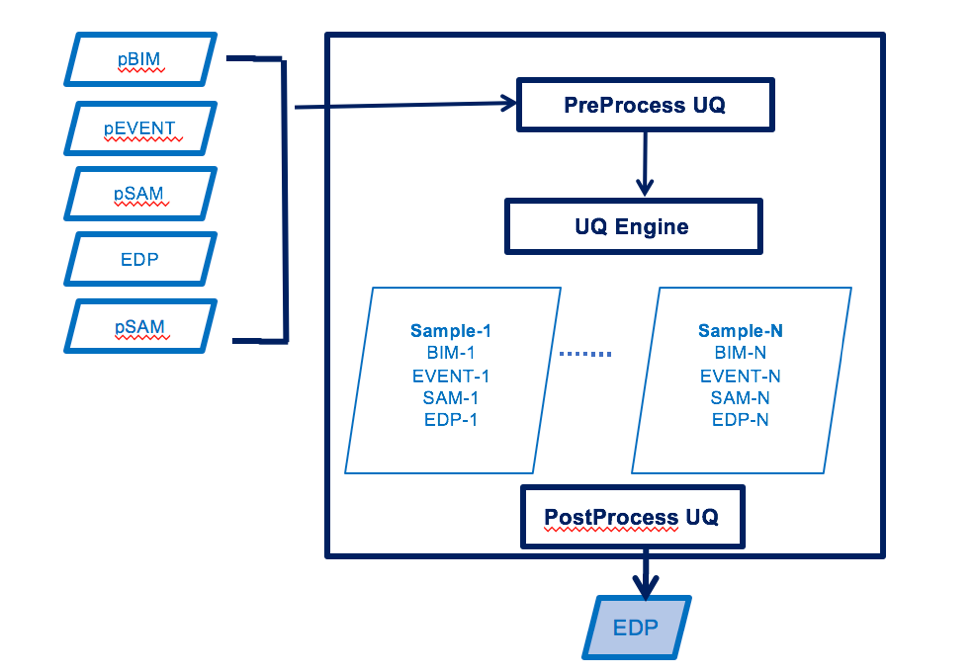
\includegraphics[width=0.8\textwidth]
    {figs/Figure19.png} }
  \caption{UQ sampling}
  \label{fig:figure19}
\end{figure}

The computationally expensive part of the simulations is of course the PerformUQ. As discussed earlier, the user has the option of running locally or 
remotely at DesignSafe. When the user selects to run the job remotely, it is actually the PerformUQ operation that is run locally. The process of setting 
up the pFiles is done locally. These files are placed in a directory (along with all other needed files) and the files are transferred to DesignSafe and then an 
Agave application is invoked to run the application on Stampede2.



\chapter{Source Code}
\label{chap:SourceCode}
This source code for the tool is released under the 2-clause BSD License, commonly called the FreeBSD license. 
It is available for download from the tools GitHub repository: \\
\href{https://github.com/NHERI-SimCenter/EE-UQ}{https://github.com/NHERI-SimCenter/EE-UQ}

\chapter{User Training}
\label{chap:training}
User Training consists of an online video available from the tool webpage that demonstrates tool use. The tool will be presented in user workshops hosted by the SimCenter. 

\chapter{Requirements}
\label{chap:requirements}
The following table outlines the user requirements identified for this tool. If you want some additional features added, contact us.

\begin{table}[hbt!]                 
  \centering
\begin{adjustbox}{max width=\textwidth}            
  \begin{tabular}{llll}                    
    \toprule          
      \# & Description & Priority & Version \\ \hline
    
      1 & Ability to perform UQ on Building with Single Earthquake &  &  \\ \hline
	1.1 & Run on Local Machine (Mac and Windows) & M & 1.0 \\ \hline
	1.2 & Run on Stampede2 through DesignSafe utilizing Agave & M & 1.0 \\ \hline
	2 & Motion Selection &  &  \\ \hline
	2.1 & Ability to select from Multiple Earthquakes and view UQ due to all the discrete events & M & 1.0  \\ \hline
	2.2 & Ability to select from list of SimCenter motions & M & 1.0 \\ \hline
	2.3 & Ability to select from list of PEER motions. & D & 1.0 \\ \hline
	2.4 & Ability to use OpenSHA and selection methods to generate motions & D & 1.0 \\ \hline
	2.5 & Ability to Utilize Own Application in Workflow & M & 1.0 \\ \hline
	2.6 & Ability to use Broadband & D & 1.1 \\ \hline
	\multirow{5}{*}{2.7} 
	& Ability to use bring motion from rock to surface through soil &  &  \\ 
	 & a)     1d soil effective stress analysis though different soil layers & M & 1.1  \\ 
	 & b)     2d bidirectional loading & M & 1.2 \\ 
	 & c)     2d bidirectional with full stochastic characterization of soil layers & M & 1.3 \\ \hline

	3 & Building Model Generation &  &  \\ \hline
	3.1 & Ability to use existing OpenSees model scripts. & M & 1 \\ \hline
	\multirow{5}{*}{3.2}  & Ability to define building and use Expert System to generate FE mesh. &  &  \\
	 & a)     Concrete Shear Walls & M & 1.1 \\ 
	 & b)     Moment Frames & M & 1.2 \\ 
	 & c)     Braced Frames & M & 2.0  \\ \hline
	 
	\multirow{5}{*}{3.3} & Ability to define building and use Machine Learning applications to generate FE mesh for: &  &  \\ 
	 & d)     Concrete Shear Walls & M & 2.0 \\ 
	 & e)     Moment Frames & M & 2.1 \\ 
	 & f)      Braced Frames & M & 2.3  \\ \hline

	3.4 & Ability to specify connection details for member ends & M & 2 \\ \hline
	3.5 & Ability to define a user-defined moment-rotation response representing the connection details & D & 2 \\ \hline
	4 & FEM &  &  \\ \hline
	4.1 & Ability to specify OpenSees as FEM engine and to specify different analysis options. & M & 1 \\ \hline
	4.2 & Ability to provide own OpenSees Analysis script to OpenSees engine. & D & 1 \\ \hline
	4.3 & Ability to use alternative FEM engine. & M & 1.1 \\ \hline
	5 & UQ - Method &  &  \\ \hline
	5.1 & Ability to Use Dakota UQ engine with the Monte Carlo and LHS methods to perform sampling & M & 1 \\ \hline
	5.2 & Ability to Use alternative UQ engines & M & 2 \\ \hline
	6 & UQ – Random Variables &  &  \\ \hline
	\multirow{5}{*}{6.1} & Ability to Define Variables of certain types: &  &  \\ 
	 & a)     Normal &  &  \\ 
	 & b)     Lognormal &  &  \\ 
	 & c)     Uniform & M  & 1.0 \\ 
	 & d)     Beta &  &  \\ 
	 & e)     Weibull &  &  \\ 
	 & f)      Gumbel &  &  \\ \hline
	6.2 & User defined Distribution & M & 1.1 \\ \hline
	6.3 & Define Correlation Matrix & M & 1.1 \\ \hline
	7 & Tool to allow user to store current configuration and reload it later & M & 1 \\ 
      \bottomrule      
                            
  \end{tabular}
\end{adjustbox}
  \caption{Features (M=Mandatory, D=Desirable, O=Optional, P=Possible Future)}             
  \label{tab:features}                 
\end{table}



\begin{table}[hbt!]                    
  \centering
\begin{adjustbox}{max width=\textwidth}            
  \begin{tabular}{lll}                    
    \toprule          
      Version & 	Release	 & Requirements \\  \hline
1.0	& Sept 2018 &	1.1, 1.2, 2.1, 2.2, 2.3, 2.4, 2.5, 3.1, 4.1, 4.2, 5.1, 5.2, 6.1, 7\\  \hline
1.1	 & Dec 2018 &	2.6, 3.2, 4.3, 6.2, 6.3\\  \hline
                            
  \end{tabular}
\end{adjustbox}
  \caption{Schedule}             
  \label{tab:schedule}                 
\end{table}

\chapter{Verification and Validation}
\label{chap:vnv}
This section provides examples of using \texttt{EE-UQ} for uncertainty
quantification of structural analysis models used in earthquake
engineering. Results of each model are verified against results
obtained using other tools.

\section{Two-Dimensional Portal Frame subjected to Gravity and Earthquake Loading}
In this example, a simple 2D portal frame model is used to verify the
results of \texttt{EE-UQ}. The model is a linear elastic single-bay,
single-story model of a reinforced concrete portal frame, as shown in
\autoref{fig:figure20}. The analysis of this model considers both
gravity loading and lateral earthquake loading due to the El Centro
earthquake (Borrego Mountain 04/09/68 0230, El Centro ARRAY \#9, 270).
The original model and ground motion used in this example were
obtained from
\href{http://opensees.berkeley.edu/wiki/index.php/OpenSees_Example_1b._Elastic_Portal_Frame}{example 1b} on the \texttt{OpenSees} website, 
and were modified to scale the ground motion record from gravity units, $g$,
to the model units, $in/s^2$. Files for this example are included
with the release of the software and are available in the Examples
folder in a subfolder called \texttt{PortalFrame2D}.

\begin{figure}[!htbp]
  \centering {
    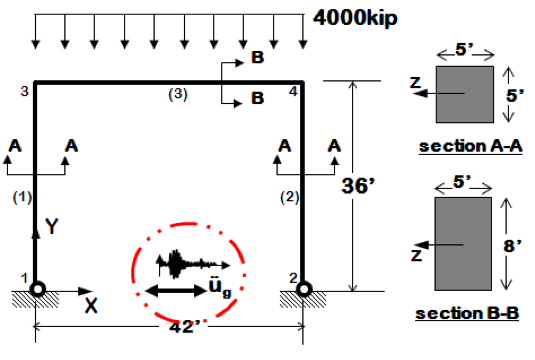
\includegraphics[width=0.8\textwidth]
    {figs/Figure20.png} }
  \caption{Two-dimensional portal frame model subjected to gravity and earthquake loading}
  \label{fig:figure20}
\end{figure}

To introduce uncertainty in the model, both mass and young’s modulus
are assumed to be normally distributed random variables with means and
standard deviation values shown in \autoref{tab:uncertainty}. In this
example, the model will be sampled with the Latin Hypercube sampling
method using both \texttt{EE-UQ} and a Python script
(\texttt{PortalFrameSampling.py}) and response statistics from both
analyses are compared.

\begin{table}[hbt!]                       
  \centering
\begin{adjustbox}{max width=\textwidth}            
  \begin{tabular}{lllll}                    
    \toprule          
      Uncertain Parameter & 	Distribution	 &  Mean  &  Standard Deviation \\ \hline
	Nodal Mass, m [kip]	 & Normal & 	5.18	 & 1.0 \\ \hline
	Young’s Modulus, E [ksi] & 	Normal	 & 4227	 & 500.0 \\ \hline
  \end{tabular}
\end{adjustbox}
  \caption{Uncertain parameters defined in the portal frame model}             
  \label{tab:uncertainty}                 
\end{table}

Modeling uncertainty using \texttt{EE-UQ} can be done using the
following steps:
\begin{enumerate}
\item	 Start \texttt{EE-UQ}, click on the simulation tab (SIM) in the left bar to open a building simulation model. Click on choose button in the input script row:

\begin{figure}[!htbp]
  \centering {
    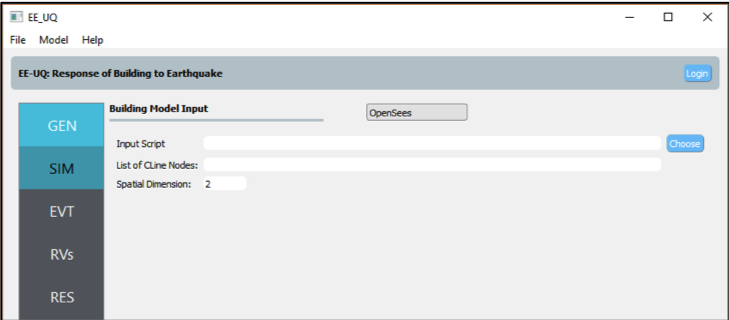
\includegraphics[width=0.8\textwidth]
    {figs/Figure21.png} }
  \caption{Choose building model}
  \label{fig:figure21}
\end{figure}

\item	 Choose the model file \texttt{Portal2D-UQ.tcl} from PortalFrame2D example folder.
\begin{figure}[!htbp]
  \centering {
    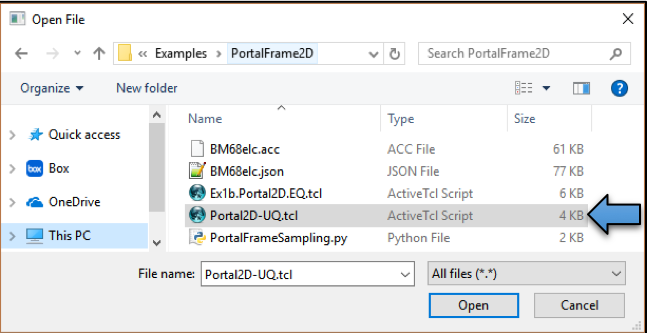
\includegraphics[width=0.8\textwidth]
    {figs/Figure22.png} }
  \caption{Choose tcl file}
  \label{fig:figure22}
\end{figure}


\item	 In the list of Clines Nodes edit box, enter “1, 3”. This indicates to \texttt{EE-UQ} that nodes 1 and 3 are the nodes used to obtain EDP at different floor levels (i.e. base and first floor).
\begin{figure}[!htbp]
  \centering {
    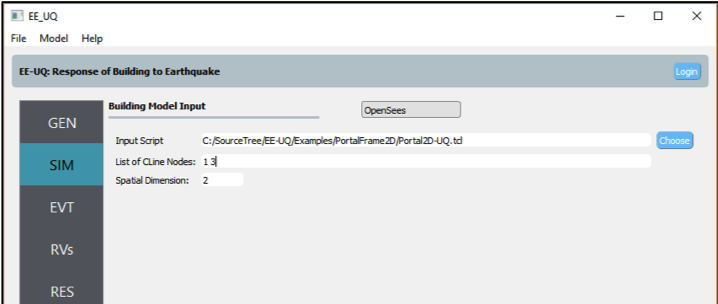
\includegraphics[width=0.8\textwidth]
    {figs/Figure23.png} }
  \caption{Select nodes}
  \label{fig:figure23}
\end{figure}

\item Click on the event tab (EVT) in the left bar to open the earthquake event specification tab, select Multiple Existing for loading Type. Click on the add button to add an earthquake event. 
Then click on the choose button to select the event file.
\begin{figure}[!htbp]
  \centering {
    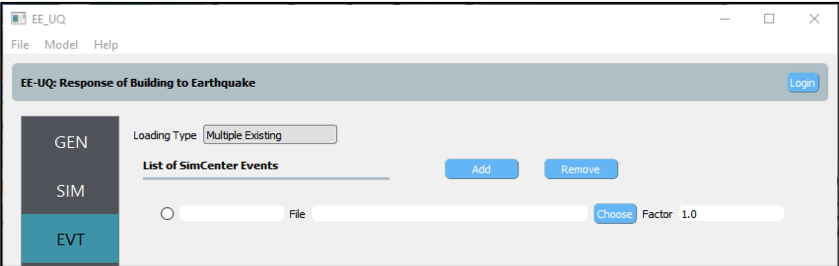
\includegraphics[width=0.8\textwidth]
    {figs/Figure24.png} }
  \caption{Work on EVT tab}
  \label{fig:figure24}
\end{figure}

\item Choose the event file (\texttt{BM68elc.json}) for El Centro earthquake provided in the portal frame 2D example folder.
\begin{figure}[!htbp]
  \centering {
    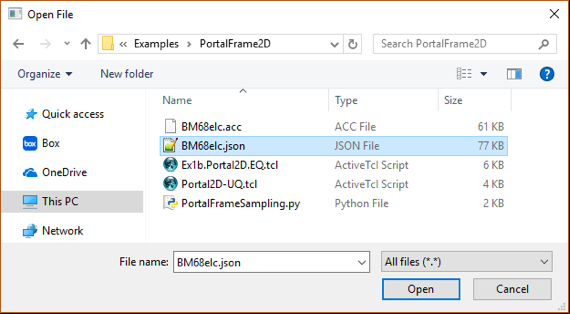
\includegraphics[width=0.8\textwidth]
    {figs/Figure25.png} }
  \caption{Choose event file}
  \label{fig:figure25}
\end{figure}

\item Now select the random variables tab (RVs) from the left bar, change the random variables types to normal and set the mean and standard deviation values of the floor mass and
Young’s modulus.  Notice that \texttt{EE-UQ} has automatically
detected parameters defined in the \texttt{OpenSees} tcl file using the pset
command and defined them as random variables.
\begin{figure}[!htbp]
  \centering {
    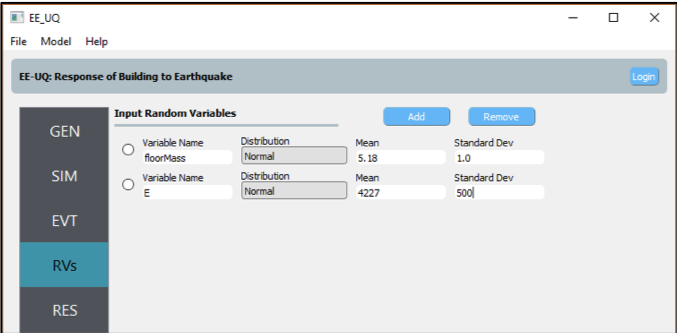
\includegraphics[width=0.8\textwidth]
    {figs/Figure26.png} }
  \caption{Work on RVs tab}
  \label{fig:figure26}
\end{figure}

\item Now click on run, set the analysis parameters, working directory and applications directory and click submit to run the analysis. 
If everything ran successfully the program will automatically open the results tab showing the summary of results (\autoref{fig:figure27}).
\begin{figure}[!htbp]
  \centering {
    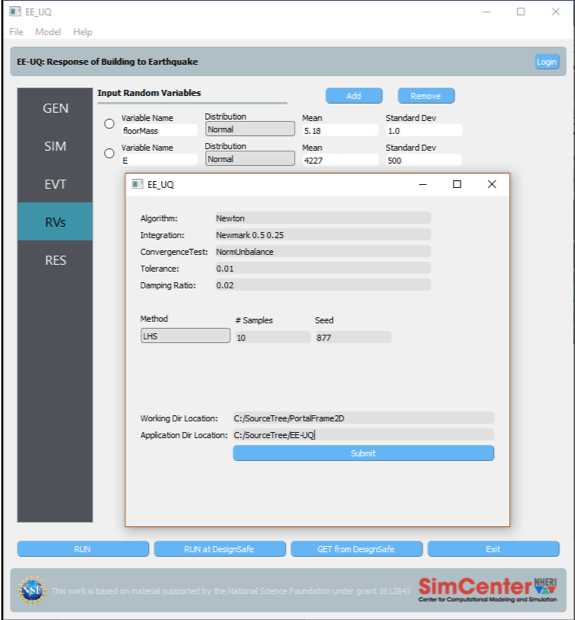
\includegraphics[width=0.8\textwidth]
    {figs/Figure27.png} }
  \caption{Run}
  \label{fig:figure27}
\end{figure}

\end{enumerate}


\subsection{Verification Script}
A verification script (Listing 1) for propagating the uncertainty was
developed in Python and is included in the example folder.  The script
creates 1000 samples for both the Young’s modulus and mass values
using Latin Hypercube sampling, then modifies the \texttt{OpenSees} model, runs
it and stores the output.  After all the model samples are processed,
the script will compute and output the mean and standard deviation
values of the peak floor acceleration and peak drift.


\begin{python}[caption=Python script for analyzing the portal frame model with uncertain parameters]
import numpy as np
import os
import shutil
import subprocess
from pyDOE import *
from scipy.stats.distributions import norm

#Setting number of samples
nSamples = 1000

#Creating latin hyper cube designs
design = lhs(2, samples=nSamples)

#Sampling Young's Modulus and Mass
ESamples = norm(loc=4227, scale=500.0).ppf(design[:,0])
mSamples = norm(loc=5.18, scale=1.0).ppf(design[:,1])

#Initializing output arrays
PFA = []
PID = []
#Reading OpenSees Model
with open ("Ex1b.Portal2D.EQ.tcl", "r") as portalFrameFile:
    portalFrameModel = portalFrameFile.read()

    #Looping through the samples and creating modified models
    for i in range(nSamples):
        sampleName = str(i+1)
        if(os.path.exists(sampleName) and os.path.isdir(sampleName)):
            shutil.rmtree(sampleName)

        os.mkdir(sampleName)
        shutil.copy('BM68elc.acc', sampleName)

        #Modifying the model using sample E and m values
        with open (sampleName + '/Ex1b.Portal2D.EQ.tcl' , "w+") as modifiedFile:
            modifiedModel = portalFrameModel.replace('pset floorMass 5.18', 'pset floorMass ' + str(mSamples[i]))
            modifiedModel = modifiedModel.replace('pset E 4227', 'pset E ' + str(ESamples[i]))
            modifiedFile.write(modifiedModel)

        #Running OpenSees
        subprocess.Popen("OpenSees Ex1b.Portal2D.EQ.tcl", shell=True, cwd=sampleName).wait()

        #Reading Peak Floor Acceleration
        with open (sampleName + '/PFA.out' , "r") as pfaFile:
            PFA.append(float(pfaFile.readlines()[2]))

        #Reading Peak Floor Acceleration
        with open (sampleName + '/PID.out' , "r") as pidFile:
            PID.append(float(pidFile.readlines()[2]))

        #Cleaning up
        shutil.rmtree(sampleName)

#Printing results
print 'Mean Peak Floor Acceleration: ', np.mean(PFA)
print 'Peak Floor Acceleration Std. Dev: ', np.std(PFA)

print 'Mean Peak Drift: ', np.mean(PID)
print 'Peak Drift Std. Dev.: ', np.std(PID)
\end{python}

\subsection{Verification of Results}
In this section, the results produced for the portal frame
by \texttt{EE-UQ} are verified against the results of running the same
problem using the Python script.  Running the uncertainty
quantification problem on the local computer produces the results
shown in \autoref{fig:figure28} Running the analysis using the
sampling Python script produces the results shown
in \autoref{fig:figure29}.  Both results (Mean and standard deviation
values of EDPs) are compared in \autoref{tab:edp} and are shown to be in good
agreement.

\begin{figure}[!htbp]
  \centering {
    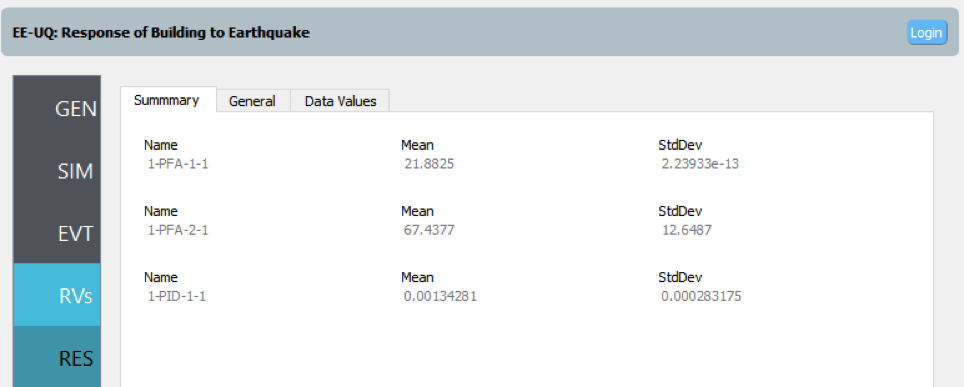
\includegraphics[width=0.8\textwidth]
    {figs/Figure28.png} }
  \caption{Outputs from \texttt{EE-UQ}}
  \label{fig:figure28}
\end{figure}


\begin{figure}[!htbp]
  \centering {
    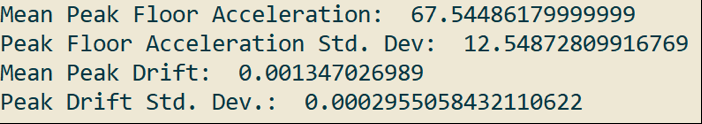
\includegraphics[width=0.8\textwidth]
    {figs/Figure29.png} }
  \caption{Outputs from PortalFrameSamplying.py script}
  \label{fig:figure29}
\end{figure}




\begin{table}[hbt!]                 
  \centering
\begin{adjustbox}{max width=\textwidth}            
  \begin{tabular}{lllll}                    
    \toprule          
      Engineering Demand Parameter &	 & \texttt{EE-UQ}	& Python Script	 & Percent Difference [\%]  \\ \hline
    
	\multirow{2}{*}{Peak Floor Acceleration [in/$s^2$]} 
	 & Mean &	67.4377	& 67.5448	& 0.16 \\
      & Std. Dev.	& 12.6487	 & 12.5487	& 0.8 \\ \hline
      
      \multirow{2}{*}{Peak Story Drift [x10-3 in]} 
      & Mean &	1.3428 &	1.347 &	0.3 \\
      & Std. Dev.	& 0.2832 &	0.2955	& 4.1	 \\

      \bottomrule      
                            
  \end{tabular}
\end{adjustbox}
  \caption{Engineering demand parameters verification}             
  \label{tab:edp}                 
\end{table}

\section{Response Spectrum Calculation using Stochastic Ground Motion Model}
The purpose of this analysis is to verify that \texttt{EE-UQ} is able
to reproduce the correct pseudo-acceleration response spectrum when
using synthetic acceleration time histories generated using the
stochastic ground motion model option as the seismic event. The maximum
pseudo-acceleration for a single-degree-of-freedom system with varying
natural frequencies calculated by \texttt{EE-UQ} is compared to the
values predicted by \texttt{smelt} as well as the geometric mean
of the four NGA-West2 ground motion prediction equations (GPMEs)
that account for soil sites. 

The single-degree-of-freedom system was input using the MDOF option as
the Building Model Input in \texttt{EE-UQ}. Here, the mass was set to
unity and the damping ratio to 5\%. The story stiffness was modified
to set the natural frequency of the system in order to calculate the
response spectrum. The structural response was calculated for 10
sample synthetic acceleration time histories for each structural
period and compared to those from \texttt{smelt} and the GMPEs, as
shown in \autoref{fig:stochastic_validation}. As can be seen in this
figure, the spectral response calculated by \texttt{EE-UQ} falls
within the mean plus/minus one sigma bounds of the GMPEs and
\texttt{smelt} while tending toward the mean. This produces the
expected result as \texttt{EE-UQ} is calling \texttt{smelt} in the
backend to generate the synthetic motions. The full validation of
\texttt{smelt} in implementing the predictive stochastic model
proposed by Vlachos et al. (2018) \cite{vlachos2018predictive} can be
found in the
\href{https://github.com/shellshocked2003/Stochastic-Loading-Module/blob/master/README.md}{library
  documentation}.

\begin{figure}[!htbp]
  \centering {
    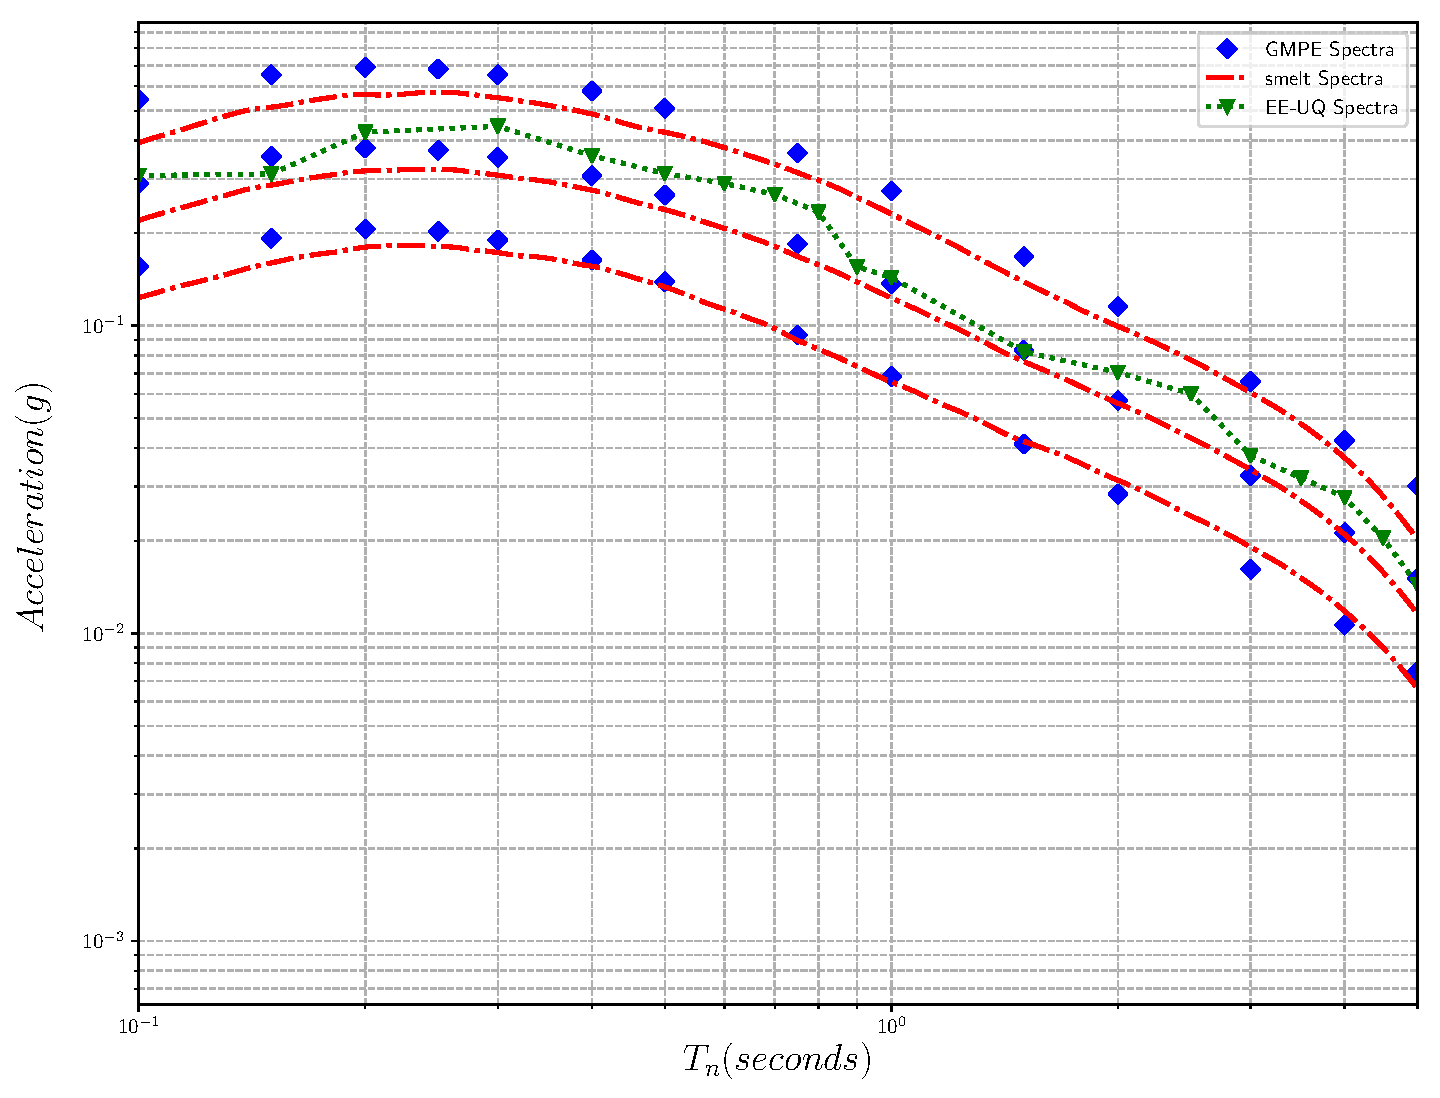
\includegraphics[width=0.8\textwidth]
    {figs/M65R20V400.pdf} }
  \caption{Response Spectra generated using NGA-West2 GMPEs,
    \texttt{smelt} \& \texttt{EE-UQ} for $M_W = 6.5$, closest-to-site
    distance $R = 20km$, and average shear-wave velocity $V_{s_{30}} =
    400m/s$. The \texttt{smelt} and GMPE spectra show the mean and
    mean plus/minus one logarithmic standard deviation. The GMPE
    spectra are based on the geometric mean of the four NGA-West2
    models that account for site soil conditions. The \texttt{smelt}
    spectra are based on an ensemble of 1000 synthetic ground
    motions. \texttt{EE-UQ} response values are based on the mean
    pseudo-acceleration for 10 synthetic ground motion samples per
    period, $T_n$}
  \label{fig:stochastic_validation}
\end{figure}



\nocite{*}

% \appendix
% \chapter{More Monticello Candidates}

\pagestyle{plain}
{
  \renewcommand{\thispagestyle}[1]{}	
  \printbibliography           
}

\end{document}